% This is the manuscript master for the [a][s] Retrospective Vol. 1.
% All LaTeX *code* is released under an MIT license.
% All *writen content* is released under a CC BY-NC-SA license, and is copyright
% the original author.  Please see the `LICENSE.md` file for more information.

\documentclass[12pt,letterpaper,oneside]{memoir}

%%% Resets
% memoir defines footruleskip, we want fancyhdr's
\let\footruleskip\undefined
\DisemulatePackage{setspace}

%%% Packages
\usepackage{fancyhdr}
\usepackage{graphicx}
\usepackage{lastpage}
\usepackage{setspace}
\usepackage{ulem}
\usepackage{wrapfig}

%%% Headers/Footers
\pagestyle{fancyplain}
\fancyhf{}
\fancyheadoffset[r]{.01in}
\fancyhead[R]{[a][s] Retrospective 2 / Makyo / \thepage\ of \pageref{LastPage}}

%%% Font
\renewcommand*\rmdefault{ptm}
\renewcommand*\ttdefault{pcr}

%%% Spacing
\onehalfspacing
\usepackage[top=1in, bottom=1in, right=1in, left=1in]{geometry}

%%% Commands
\newcommand\secdiv{
  \begin{center}
    \#
  \end{center}
}
\newcommand\articlehead[3]{
  \newpage
  \section[#1 \textit{(#2)}]{#1}

  \begin{center}
    \textit{Copyright \copyright\ #3 #2; licensed under cc BY-NC-SA 3.0}
  \end{center}
}

\begin{document}
  \title{[adjective][species] Retrospective Year 2}
  \author{Madison ``Makyo'' Scott-Clary, \textit{Ed.}}
  \maketitle
  \newpage

  \tableofcontents

  \part{Introduction}
  This volume contains the major articles posted in the first year of [adjective][species].

Reh SoFurry con yap wolf, bark anthrochat FurAffinity headless fur Midwest Fur Fest. Furnation tailswish bark whiskerflick VCL wiggle SPR tapestries yip anthrochat, wag. Bark Midwest Fur Fest fox, bark popufur Midwest Fur Fest wag fox wolf Midwest Fur Fest Yerf! wolf FA. Ott whiskerflick taps tailswish FurAffinity mew, fursuit ruining the magic SPR meow wiggle otter sergal otter furries. Booper, furcadia popufur tapestries AC Midwest Fur Fest furnet fox growl fox. Weasyl ruining the magic anthrochat popufur furnation whiskerflick taps feesh, mew icon anthrocon pet commission squeak, MFF growl SPR reh Weasyl ruining the magic SPR Midwest Fur Fest husky, sergal commission icon commission Yerf! popufur. Taps tapestries meow furnet.

Swish stream anthrochat Yerf! fur Weasyl fur squeak murr, FurryMUCK anthrocon, feesh otter FurryMUCK swish VCL tapestries Further Confusion SoFurry furries. VCL boop reh. Ruining the magic murr headless SPR Yerf!. Meow anthrocon anthrocon icon ruining the magic, cat Wikifur. Feesh furries icon tapestries furries wolf furries, husky ruining the magic fur con furnation tailswish sparkledog, Yerf! yap suiter anthrocon meow. Fox cat AC bark. Weasyl booper con AC boop ott, cat furnet SPR ruining the magic.

Sergal sparkledog headless sketch booper, con popufur swish pet furre ruining the magic sergal Midwest Fur Fest FA, tailswish con headless FurryMUCK feesh. Otter SPR VCL pet wag commission InkBunny fursuit wolf, ruining the magic furre convention. Icon swish boop otter furry, anthrochat Midwest Fur Fest whiskerflick Midwest Fur Fest, mew FurAffinity growl sketch stream fox furries sergal Further Confusion meow Yerf!. Ruining the magic anthrochat bark ott booper Further Confusion AC fursuit, growl furries cat MFF cat husky feesh tapestries anthrochat whiskerflick, convention boop pet sketch popufur Further Confusion. Con FurAffinity cat mew FurryMUCK, Midwest Fur Fest wiggle icon SoFurry yap SoFurry SPR taps, cat suiter sketch stream feesh meow yap furnet husky, con AC FC furre wiggle. Cat anthrochat InkBunny growl ott popufur wiggle, pet headless headless reh fox growl pet stream, headless reh. FurryMUCK anthrocon FA furre yip, pet Yerf! squeak taps Midwest Fur Fest icon husky taps SoFurry.

MFF furcadia Further Confusion, VCL boop sergal husky. Wag, sparkledog taps murr furry, Yerf! commission FurAffinity popufur fursuit. Ott, headless. Furry fox feesh Further Confusion commission booper VCL furry SPR mew. Pet FurAffinity tapestries, whiskerflick boop popufur furre FurAffinity, Wikifur murr FA pet. Furre yip, bark yap. Whiskerflick Wikifur FA.

Squeak furre boop AC whiskerflick AC furnation mew reh, taps FC fox suiter sergal boop wolf swish stream. MFF meow convention Midwest Fur Fest fursuit SoFurry. Sketch stream boop furries commission fur InkBunny headless AC boop, AC swish sparkledog tailswish, FA fursuit sergal FC booper. Bark furre icon commission SPR VCL cat, meow fox suiter boop, furnation swish sparkledog. Reh FA Yerf! reh tailswish con booper yip furnation. Ruining the magic Midwest Fur Fest FurAffinity anthrochat furries growl anthrocon Weasyl con, SoFurry, icon sketch growl furry fox ruining the magic feesh furre wiggle. Wag taps FurAffinity, scritch growl con growl SoFurry, AC anthrocon Weasyl tapestries.


  \part{The [adjective][species] Retrospective, Year 2}
  \chapter{November}
  \articlehead{Furries With Physical Disabilities}{JM}{2012}

For many furries, there are big physical differences between their real-world bodies and their preferred avatar. We often act as if our animal-person representation really exists: we might consider the logistics of tails, we might miaow or bark a greeting, we might assume personality traits that reflect our perception of our species.

Such roleplay is central to the furry experience for many people. Online, furries commonly present as their animal-person avatar and will socialize as if everyone else were their fursona. This behaviour translates, to an extent, to real-world furry spaces, from one-on-one meetings through to conventions.

This `fursona illusion' occurs regardless of how closely our real body matches our avatar. For those furries who feel their real-world body doesn't reflect their self-image, this can be a liberating experience. And for furries who are physically disabled -- perhaps wheelchair bound -- it has the potential to transcend their disability.

People who are physically disabled have a challenging life. Most obviously, they may be physically restricted by a society that is set up for the able-bodied. However restrictive, this is less of a problem from a mental perspective, and more a logistical puzzle that needs to be solved. This is particularly the case for those who are congenitally disabled, and so experience physical restrictions as `normal'.

More subtly, and more importantly from a mental point of view, is that physically disabled people are treated differently by able-bodied members of society. Anyone who physically presents in an unusual fashion -- weight, race, clothing, anything -- will tend to suffer from the same prejudice, where other people become unsure of how to engage in social contact. This is not to place blame: it is simply human nature. (I'll discuss the psychology of this prejudice a little further down.)

Research shows that the well-being of the physically disabled is strongly correlated with their sense of community engagement. Efforts to improve the lives of the physically disabled therefore often focus on social aspects. This is the target of public awareness campaigns with slogans like ``see the person not the disability''.

Furries pay less regard to physical appearance. We are used to treating fellow furs as if they were their animal-person avatar. The furry world, then, may provide a social environment where physically disabilities are less relevant.

I chatted with three physically disabled furries who were happy to share their experiences inside and outside the furry community. These conversations took place over text and are edited for clarity and length.

\textbf{BlooCat} (IBloo on Fur Affinity) is a UK fur with muscular dystrophy and a wheelchair, who might be described as a garden-variety furry:

\begin{quote}
  My fursona is just a cat representation of myself. By that I mean she shares my name, age, personality etc. Having my fursona do things I can't do is fun, but sometimes I don't like it because it feels less me. My disability isn't all I am, but it's also not something I feel that I want to get rid of.
\end{quote}

BlooCat's physical disability is obviously restrictive, and she finds that people are often unsure of how to react when she meets them. This awkwardness is also experienced by \textbf{Shorebuck}, an Australian fur who is very mildly disabled -- he has diplegia, a form of cerebal palsy. He isn't physically impaired in any significant sense and doesn't consider himself to be disabled, however his diplegia affects his gait, ``giving off the appearance of a limp -- or dancing''.

Despite the irrelevance of his condition from a physical point of view, Shorebuck still suffers:

\begin{quote}
  Socially, it affects a lot. Some people have been freaked out by it, and some couldn't give a crap. Some people look away when they see me.
\end{quote}

The story is similar amongst the more severely disabled. \textbf{Nornhound} is wheelchair-bound fur with a rare condition called Fibrodysplasia Ossificans Progressiva (F.O.P.), which causes painful unnecessary bone growth in her muscles.

\begin{quote}
  To a complete stranger, I am certainly known as `the disabled kid/teen/adult woman', and these strangers treat me differently from an able-bodied person. When I was in my early teens, strangers would automatically assume I had an intellectual disability, and treat me as such. They were often hostile, too.
\end{quote}

This initial awkwardness doesn't occur in the online world: physical disabilities become invisible and, from a social point of view, mostly irrelevant. The internet also provides tools that can reduce the logistical challenges posed by an able-bodied society, such as online shopping, and opens different employment opportunities. Largely due to these factors, research shows that the internet improves the wellbeing of the physically disabled (Ref).

It's not all good news. As will be clear to anyone who has spent time reading forums and comment threads, the internet can be corrosively negative. This has a greater than average impact on physically disabled people, because they are more likely to rely on the internet. Furthermore, use of the internet for escapism -- such as online gaming -- also has a negative impact on the wellbeing of the physically disabled (Ref).

From this research, it can be inferred that the online world provides the greatest benefit to the physically disabled when it is social and enjoyable. The furry community may provide this, and more -- the online furry world translates, in part, into the real world, because of the persistent `fursona illusion'. If you are physically disabled, engagement with the furry community may lead to a better offline social experience, because furries will tend to see the animal-person alter ego.

BlooCat:

\begin{quote}
  The physical barrier is more easily overcome with furries. I find a lot of non-furries are a lot less tactile with me than they would be with other people. Something that really struck me at a recent convention was the amount of people (even strangers) that would come up and ask for a hug.
\end{quote}

Shorebuck:

\begin{quote}
  I'd say the furs just accepted me [as an arctic fox named Shorebuck] -- that was the main focal point. `You are this fur, pleased to meet you.'
\end{quote}

The initial awkwardness experienced by many people when meeting someone physically disabled may be less common among furries, but it still exists. This is an unavoidable outcome of our human nature as social beasts.

In the furry and non-furry worlds, social groups tend to act as a kind of meritocracy. We tend to socialize with our peers: people who occupy a comparable position in life. The process of peer group selection is driven by our desire to `fit in' -- we tend to change our own behaviour towards the group's behaviour; outsiders who meet or exceed the group's standards are welcomed; outsides who fail to meet the group's standards are rejected.

This phenomenon of normalization is clearly demonstrated by a 2007 study that tracked the incidence of obesity within social groups over a long period (Ref). The results showed that social norms have a very significant impact on obesity risk: essentially, that fat people tend to have fat friends. The results do not strongly suggest (as was reported in the media) that having fat friends can cause you to be fat; more that fat people are likely to find and keep equally generously-proportioned friends.

Such normalization of peer groups occurs everywhere in human society, with the criteria varying depending on the nature of the group. At its simplest level, people tend to have peers that are a similar age. To choose a few examples from the furry world: skilful artists are likely to hang out together, strong programmers are likely to hang out together, and furries with similar sexual interests are likely to hang out together.

This unsaid enforcement of social norms is a natural process, but it can have negative consequences if you are different. Furry is a broad church -- geekiness, gayness, intelligence, introspectiveness, etc -- and accordingly many furry readers of this article will be familiar with how someone different can fail to `fit in' to a social group. Or, to put it another way: the girl in the wheelchair isn't going to catch the eye of the captain of the football team.

The feeling of awkwardness felt by many when meeting someone physically disabled is normal. It is rooted in the same psychological phenomena that lead to peer group normalization. When we meet someone unusual, we are unable to draw upon on an unconscious `social script' that we use with our regular peer groups. This causes us to engage our conscious mind: we ask ourselves ``what should I say''. This leads us to think about how we are being perceived (psychologically, we become `self aware'), which can make us awkward and anxious. It's the same process that makes teenage boys nervous around teenage girls.

These feelings of anxiety are unpleasant and can provoke someone to withdraw from a conversation. This is frustrating for the physically disabled person, who sees it all the time. Unfortunately there is no easy way to overcome this initial conversational hurdle, no fallback social script.

BlooCat:

\begin{quotation}
  I know it would be a lot easier if there could be a set script, but it's a very personal thing. What I think is okay, someone else may not agree with. Take for example another girl in a wheelchair I know, we had a discussion about how we feel about people touching our wheelchairs when we're in a bar or something. Her view was that it shouldn't be touched as it's your personal space. For me I don't really mind if someone leans a bit on my chair, it's just a chair. A fancy bar stool even.

  The same applies for when you meet a disabled person for the first time. I think people just need to disregard the disability/wheelchair. Think of it as meeting a person rather than a disabled person.
\end{quotation}

  \articlehead{Furry as an Alternative to Religion}{JM}{2012}

Furries are a diverse bunch.

Our diversity means that we're often excluded from the mainstream. This is particularly evident in our sexual preferences -- only about a third of us identify as `heterosexual' or `mostly heterosexual' (Ref). Other traits displayed by some furries -- gender dysmorphia, heavy internet usage, or even simple geekiness -- can also play a part in our diversion from society's definition of `normal'.

Not surprisingly, furries do not closely embrace religion, a societal construct that can embody and tacitly enforce the norms of the mainstream. A little more than 50\% of furries are essentially areligious (Ref). This rate is about five times higher than for the wider American population (Ref).

Furry provides some of the benefits of religion -- I identify two in this article, loosely defined as `spirituality' and `community' -- that provide insight into how mainstream society might react to the challenges of our changing world. Furries embody some of the biggest challenges to religion in the twenty-first century: acceptance of diversity, the growing online world and, most importantly, the increasing rejection of religion altogether.

Religion is rightfully a sensitive and important topic. But before I go any further, I want to make two pre-emptive apologies.

Firstly, an apology to the religious, who may reasonably find this article offensive. I'm making a direct comparison between furry and God. To suggest that something as trivial and fleeting as furry can, and should, be compared to a deity would be ludicrous if I wasn't so sincere about it. And possibly even worse, I'm also making an unsaid comparison between this article here on [adjective][species] -- my interpretation of furry's morals -- and a holy book -- a divine interpretation of God's morals.

Secondly, an apology to the atheists, who may reasonably find this article condescending. Religion is an imaginary construct, so it's ridiculous to give it any sort of regard beyond lip service. I'm being respectful towards belief systems that are demonstrably false instead of talking directly about the topic at hand.

These competing paradoxical reactions make writing this article potentially a lose-lose situation. It's also one of the reasons why religion is such a difficult topic outside of conversations with like-minded people. The godly and the godless often see each other as the enemy: they respectively speak in ways that insult the other's philosophy. It's fertile ground for misunderstandings and angry escalation.

This article is intended to explore how our ad hoc furry community provides support to its adherents in much the same way as religious communities. I am not exploring theology.

For starters: furry is not a religion. As far as belief systems go, furry is reasonably comparable to totemism, a broad term covering those who believe they have a connection or kinship with a non-human animal. Totemism has been documented largely in indigenous populations in North America and Oceania, and a modern version of it still exists.

Modern totemists will often identify a `spirit animal', with whom they feel a close personal connection. That spirit animal is usually imbued with superpowers that give strength to the totemist. These powers are often described as a result of the animal's existence in a spirit world, from which they can provide guidance or provide literal physical support to the totemist.

Modern mainstream totemism (sometimes called animism) is considered to be a “new age” philosophy, along with other artifices appropriated from a range of cultures. Your patience for such quasi-spiritual guff will vary: your reaction to the usefulness of dreamcatchers, or perhaps your thoughts on the wisdom (or otherwise) of Chakotay from Star Trek: Voyager, might be a good guide as to whether totemism is for you.

If it sounds like I'm unfairly poking fun at modern totemism, I'm also poking fun at myself. I'm personally inclined towards a lot of this new-agey stuff -- I'm vegetarian, I meditate, I'm a hypnotist, I own a lot of ambient music -- although I would argue that I've appropriated useful aspects of newageism and discarded the dreamcatchers. I've read a fair bit on totemism and I wish I could recommend a good reference -- probably the least worst is Ted Andrews's Animal Speak (link), although there is a lot of nonsense to wade through, such as the author's insistence that his personal eagle totem can disable highway speed cameras. If you can tolerate such intellectual bankruptcy, then the book is otherwise a pretty good reference for furries looking to reflect on their relationship with their species of choice. You could, unfortunately, do worse.

Having said that, totemism and real religions -- and furry -- help us manage our inner world. The totemists and the religious both provide an `other' -- a spirit animal or a God -- that allows us to explore the most difficult aspects of the human condition. At the simplest level, using this `other' as a sounding-board makes it easier to negotiate a route towards happiness, or acceptance of mortality, or manage personal failure. The presence of this `other' means that we do not have to carry the mental load of complete personal responsibility.

For the areligious, furry provides an alternative for managing our internal world.

All human beings carry around an internal critic that thinks and acts in a way that is often contrary to the rational, moral being we imagine ourselves to be. We all hear an internal voice that reminds us of our permanent failure to live up to our own expectations. We all secretly struggle with depression, or lovesickness, or anger, or mortality, or whatever our own inner voice's favourite topic happens to be.

This inner voice is believed to be the cause of auditory hallucinations. People who `hear voices', as is commonly associated with schizophrenia, may simply feel that their inner voice isn't their own. Among the rest of us, our inner voice can still make itself known. We may find ourselves acting on otherwise repressed impulses when we are in a mentally delicate state, perhaps drunk or under stress.

The struggle to manage this conflict between our inner voice and our desire to be a perfect rational being is, for many philosophers, at the core of the human condition. Some people might over-manage their atavistic impulses and become uptight, while others might under-manage and become emotionally unpredictable.

To a religious person, a deity often represents a perfect and unattainable ideal who rewards those who try to improve themselves. This provides a motive force for the internal struggle, providing meaning as one strives towards self-improvement.

Our furry selves may help in a similar fashion. For many furries, the animal-person alter-ego represents an unattainable ideal, mentally and physically. Other furries may imbue their avatar with desirable qualities, and roleplay as a first step towards self-acceptance. The fact that our avatars are not human may be helpful, in that we can never feel like we have reached our destination, much in the way that a man can approach but never attain godliness.

Furry also provides social guidance. We do not have anything as formal as a set of commandments, but we're still subject to unsaid norms that inform the boundaries of appropriate behaviour within the community. For example: furries place great value on tolerance; our friendships are more intimate; we talk freely about sex and sexuality.

These unsaid furry standards are explored regularly here at [adjective][species]. However they are difficult to pin down: I suspect that a non-furry reading these pages wouldn't gain much understanding about what furry `is'. In general, we tend to discuss common experiences (Rabbit on Fursuit Magic) or explore unusual phenomena (Makyo on furry's dearth of women, Eighty-Twenty) but we tend not to try to define `furry'.

It's not through lack of trying, just that we furries aren't easily categorized. I might propose, for example, that all furries have an animal-person alter-ego, that we create and name a furry reflection of ourselves. However this is neither mandatory nor universal -- [adjective][species]'s very own Rabbit, aka Phil Geusz, doesn't interact through an imaginary furry representative. (Having said that, his books are very `furry', particularly so if you are inclined towards bunnies.)

We have also explored apparently simple topics, like species selection. Assuming that, say, furry wolves must have different motivations for species selection from furry foxes, we hoped to find evidence in the Furry Survey data. However several creative data-mining attempts have discovered almost nothing. I can think of exactly one significant correlation related to species: furry women are much more likely to choose a domestic cat for their fursona. (Ideas for future searches are welcome.)

The spiritual aspects of religion are difficult to pin down as well. Taking Christianity as an example, the world has changed to a point where the bible has ceased to be a realistic reference for behaviour. (Atheists sometimes suggest that failure to adhere to the word of the bible is proof that it's at least partly false. I suspect that Christians roll their eyes at this criticism.)

The world is always changing, a process that become very rapid following the industrial revolution some 200 years ago. Huge increases in efficiency and income have led the world's population to increase from about 1 billion to today's 7+ billion, largely away from rural communities and into urban centres.

Religion has had to adapt to this change. Before cities started growing in the nineteenth century, people related to their religion at a community level. The church was at the heart of the community, a role perhaps comparable to that of the government today (as illustrated by the Soviet Union's attempt to enforce universal atheism).

Population growth and the rise of the cities has changed religion. The paradigm of a community church has foundered in the wake of cultural diversity, social diversity, and -- more recently -- the advent of the internet. Furry is less than 30 years old and so has easily adapted to the twenty-first century. Most religions have centuries or millenia of history: they were once described to me as like an oil tanker, in that they take a long time to change course. By that metaphor, furry would be a speedboat.

While the spiritual aspects of religion haven't appreciably changed over this time, the community that once centred around a church has. In diverse cities, church-based community will necessarily be relatively monocultural compared to the greater population. This disconnects you from your citymates, a disenfranchisement from society.

If the inhabitants of a city are not engaged with one another, it can lead to weakening of the social contract. This causes problems on a personal level -- a city can be lonely -- and on a wider level -- illustrated by the 2011 London summer riots. The furry community provides a solution, at least on a personal level.

Our mutual engagement in the furry community brings us closer together. The social contract within furry is strong: we freely offer shelter and company to furry strangers (The Furry Accommodation Network); we offer moral support to the depressed (A Rough Guide to Loneliness); when furry strangers pass away, we are personally affected and provide charity (Death in the Fandom). This sense of community is very similar to that traditionally provided by religion, bringing an entire community together, allowing the strong assist the weak.

The communal furry experience is more tangible than the spiritual side. Unsurprisingly, we at [adjective][species] regularly write about the furry community's actions, and those articles are almost always the most interesting to read. So, if you've read this far, thanks -- I hope you didn't just read to the end so you can comment and berate me for being offensive/condescending [choose one].

  \articlehead{Carroll Ballard's \textit{The Black Stallion}}{JM}{2012}

\textit{The Black Stallion}, Carroll Ballard's 1979 debut feature, is a great film.

It's based on a series of children's books but isn't simplistic or pandering. It's meditative, beautiful, engaging and -- of course -- great for any furs with an affinity for our equine friends.

The movie opens with a young boy, travelling on a foreign ship with his father. The ship is carrying the titular black stallion, a beast with a questionable temperament and unquestionable power.

There is a storm. The boy frees the horse from its restraints before both are thrown overboard. The ship sinks. They find themselves on a deserted island as the only apparent survivors, marking the end of the prologue and the beginning of the movie proper.

The first half of the film is a nearly wordless tale of survival. The weathered pastels of the island and the primary blue of the ocean are stunning. This landscape acts as an ancient canvas for the emerging relationship between boy and horse.

Ballard allows the story to develop naturally, with long scenes showing the boy adjusting to his wild surroundings. Such unhurried minimalism is comparable to the quiet, tense scenes of exploration in \textit{2001: A Space Odyssey} (1968): the boy's quest for survival has parallels in Kubrick's apes discovery of tools, or Floyd's moonwalk to the excavated monolith, or Bowman's slow discovery of Hal's treachery. Like Kubrick, Ballard simultaneously evokes tension and wonder with \textit{The Black Stallion}, although never with the thematic reach or artistic pretension of 2001.

The second half of the film, following the rescue of the boy and the horse, is less effective. But more on that in a moment.

The relationship between the boy and the horse is one of codependence. The boy is saved from probable death twice by the stallion. Firstly, after being thrown overboard from the ship, the boy grabs the horse's restraints and is carried to the safety of the island. Secondly, on the island, the horse tramples an aggressive snake.

The boy saves the stallion from probable death twice. He frees the horse from its restraints on the ship and again on the island, where the horse becomes trapped in a rocky outcrop.

The growing trust between the two leads to \textit{The Black Stallion}‘s best scene, where the boy attempts to feed the horse by hand. If I can anthropomorphize the horse for a moment (and I'm sure readers of [adjective][species] won't mind), I'd argue that this scene shows the greatest acting performance ever by a horse. It is certainly a triumph of animal handling. The horse is clearly nervous as he approaches the boy, pushed and pulled by the competing emotions of anxiety and hunger. His slow approach to the boy's offering is filmed from a distance: a long single shot. The scene is amazing and natural and joyful.

The boy and the horse, doomed to early death alone, combine to thrive on the island. The horse's power provides a blunt instrument against the forces of nature, protecting them both from danger. The boy's resourcefulness helps them survive day-to-day, providing food and shelter. The boy is rightfully fearful of the highly-strung stallion initially but, as the two help one another, respect grows into trust which grows into a tight bond.

The scenes showing the friendship between the boy and the horse are my favourite in the whole film. The two, agents of one another's needs, start to find island life easy. They play: they swim together and the boy (eventually) learns to ride the stallion. These scenes -- the stallion's enthusiasm and the boy's laughter -- wordlessly depict the joyfulness of their bond.

From a less life-affirming perspective, it's possible to interpret the stallion as an agent of death. In the film's chronology, he seems to be the arbiter of who lives and who dies. Ballard's films often starkly depict death, and this is the case in \textit{The Black Stallion}, which opens with the death of the boy's father and presumably the rest of the ship's passengers and crew.

The boy survives the shipwreck because his obsession with the horse draws him to deck to cut the stallion's restraints. As the horse jumps overboard, the boy is tossed over by the storm, saving him from the boat's subsequent explosion. Later, after the boy frees the horse from his tangle in the island's rocks, the horse saves the boy from the snake. In both cases, the boy's survival is directly associated with -- and arguably caused by -- his selflessness towards the stallion. The horse, as Death, shows mercy towards those that show mercy to him.

The same events could, of course, be interpreted as a representation of the power of friendship. However I prefer the horse-as-manifestation-of-Death theory, and I point towards the stallion's black coat as evidence.

It might be a stretch to suggest that \textit{The Black Stallion} is an exercise in karmic vengeance, but the horse is shown to be wild, powerful, and dangerous. In an early scene on the boat, the horse is shown fighting against his handlers as they corral him into his stall. The boy is fascinated by the stallion's power and becomes drawn to him, firstly by supplying illicit sugarcubes, and ultimately cutting him to freedom in the storm.

On the island, the horse is still dangerously flighty. However the boy's obsession means he does not see the horse as a threat, and his persevering kindness is rewarded. Their friendship endures when the boy is eventually rescued: the horse swims out to the boat, convincing the rescuers to bring the horse on board as well.

Back at home, the boy is reunited with his grieving mother, and the movie becomes a different beast. The stallion escapes from their yard; the boy meets possibly the most egregious magical negro in cinematic history (who comes with magical and totally gay horses); the horse is found in the barn of a retired jockey; they enter into a horse race for no obvious reason other than to give the film a convenient, and clichéd, climax.

The retired jockey is played by Mickey Rooney, who is most famous for hamming it up as a cherub-faced child actor in the 1920s and 30s. His brand of ham has aged poorly, and his scenes in the \textit{The Black Stallion} are the worst of the film. (Kelly Reno, as the boy, comfortably out-acts one of the most celebrated child actors of all time.) While researching this article, I was shocked to learn that Rooney was nominated for an Academy Award for \textit{The Black Stallion}. It must have been a sympathy vote. He did not win.

For all the lameness of the second half of The Black Stallion‘s plot, it is still a beautiful film. The small town in which the boy lives is a perfect slice of rural America. And there is a racetrack scene -- a reporter is invited to see the stallion go through his paces -- set in a night-time cloudburst that stands alongside the best moments of the film.

In this way, the cinematography of \textit{The Black Stallion} is comparable to the craptactular films of Michael Bay (\textit{Bad Boys}, \textit{Pearl Harbour}, \textit{Transformers}). Bay's films may be irredeemable nonsense, but they are beautifully shot. A Bay film, randomly paused, will often be composed and striking. (It's a pity Bay and his team don't put as much effort into the plot, direction, continuity, or assessment of his audience's intelligence.) \textit{The Black Stallion}, even in it's lowest Rooney-filled moments, is always pretty.

The climactic race scene of \textit{The Black Stallion} is almost Bay-worthy in its preposterousness. However the horseback scenes, shot largely in close range around the boy and the horse, are vivid and moving in their depiction of the stallion's speed and power. A similar technique is used in \textit{The Club}, a 1980 film that follows an Australian Rules team. By filming close to the players and bringing their footfalls to the front of the sound mix, the viewer gets a visceral sense of the footballer (or horse) testing himself to his thoroughbred limits. These scenes, in \textit{The Black Stallion} and in \textit{The Club}, share the athlete's perspective with the viewer like no other.

Notably, and laudably, \textit{The Black Stallion} is not a coming-of-age story. The boy is shown to be self-reliant from the beginning of the film but is very much a child throughout. His journey, starting with the death of his father and ending in a horse race, is defined by his relationship with the horse.

Both boy and horse are juvenile. They complement one another and help one another survive, thrive, and succeed. The boy is creative and the horse is powerful: they are, each, half a man. Together they are a match for the world.

\textit{The Black Stallion}, then, is a celebration of childhood. One day the boy will grow and become strong and powerful himself, and he will no longer need his other half, the horse. However this is not the subject of the film. In \textit{The Black Stallion}, both boy and horse are free to enjoy and explore their childhood, through their friendship.

\secdiv

This is the first of four posts on the films of Carroll Ballard. The other three articles will come irregularly, as I write them. All four movies are great. Choose your species and join us:

\begin{itemize}
  \item \textit{The Black Stallion} (horse)
  \item \textit{Never Cry Wolf} (wolf): coming soon
  \item \textit{Fly Away Home} (goose): coming soon
  \item \textit{Duma} (cheetah): coming soon
\end{itemize}

  \articlehead{How Being a Furry Saved Me Forty Grand}{Rabbit}{2012}

Tonight I test-drove a \$40,000 pickup truck. Don't get me wrong—I never had the slightest intention of buying the thing. As I made sure the salesman knew before I ever climbed in and turned the key, I was actually maybe, possibly interested in a baseline truck that costs about half that. My current plain-jane 4×4 is seventeen years old and has nearly 100,000 miles on it, you see, and the auto manufacturer I work for is currently offering large rebates to the general public and even larger ones to their employees to move the things more quickly, which sparked my interest. But the dealership had nothing but top-end super-fancy (read that ``high margin, high profit'') stuff on their lot, so if I wanted to take a test drive it was a \$40,000 truck or nothing.

The trip around the test loop was routine, including the salesman establishing who I worked for and thereby learning how much he might be able to bleed me for. I told him, of course—it's not polite not to. So when we returned to the dealership I was treated to the predictable chorus-greeting from the rest of the otherwise-unoccupied sales staff. ``Oh, isn't that a gorgeous truck?'' ``I've never seen such a wonderful shade of blue!'' ``I hear (insert local celebrity's name here) drives one just like that!''

At this point of course I sighed, explained that I was still doing research, and left a terribly disappointed group of middle-aged men behind me. But in much the same way that I'm certain the salesmen, being salesmen, are still reassuring each other that I'll be back even as I type this, as a writer I find myself analyzing both their and my behavior over and over again.

(Please, give me a little more time. This article will become relevant to furry before it's over, I promise!)

The salesmen were doing their best to apply social pressure to me, to make it clear that buying a \$40,000 truck is a behavior smiled upon by society and sure to make me more popular and celebrity-like. They flattered its new-for-2013 color—I'm sure they could care less, if forced to be honest—and extolled the virtues of a product they knew for fact was a far more expensive vehicle than I really wanted or needed. Some of them—the sales manager and my own salesman—stood to profit financially if I succumbed to the pressure. But most of those doing the cajoling would gain nothing more than a smile of approval from their boss and atta-boys from their coworkers if I'd bought the silly thing.

Sadly, I'm no longer either much saddened or shocked when people treat each other as mere cash cows while conducting business. Greed explains much, and the social status associated with ``success'' most of the rest. What I can't get over is that simpleminded, transparent tactics like this continue to work and work and work, not just year after year but century after century. I mean\ldots  It wasn't just obvious to me what was going on, it was sickeningly obvious. Yet the staff wouldn't continue to behave in such a manner if it didn't sell \$40,000 trucks, and as further evidence I'm forced to acknowledge that an awful lot of my co-workers do in fact park very similar vehicles right alongside my far-cheaper one every day of the week even though they can't afford them any more than I can. In fact, they often buy them from that specific dealer and tell me afterwards what a nice bunch of guys they are!

People are so stupid, I muttered sadly to myself as I drove away from the dealership in my seventeen-year-old, still perfectly serviceable truck that not one but many salesmen have done their level best to part me from. So primitive and easily led. Then, strictly as a mental exercise, I listed those friends of mine who I reckoned might see through the sales pitch as easily as I did.

Almost every one of them was a furry, I realized with a bit of a shock.

And that's the realization that led me to pen this column. I've long contended that the furry fandom (along with the SF fandom and some others) really is different from the bulk of society in some basic, fundamental ways. Part of it is clearly intelligence—statistically speaking I believe we're well offset towards the high end of the curve—and one aspect of seeing through traps like the one at the pickup dealer is indeed intelligence. Another, I would contend, is imagination. In order to see the hidden poison behind all the happy-faced affirmation, one must first be able to imagine the possibility that such nastiness actually exists.

I believe, however, that another factor counts for more than either of these: our sense of ``outsidership''. The application of social pressure is an ineffective lever at best when applied to a dedicated non-conformist, and is often actively counter-productive. But ``normal'' people are different. From the outside looking in, at least, their need to ``fit in'' appears to be one of the most powerful forces if not the most powerful force in the lives of most non-fen. Not only does the vast bulk of the population share precisely the same short list of ``acceptable'' interests and hobbies with each other, they often grow acutely uncomfortable at so much as the idea of, say, owning an unusual species of pet or driving a car that looks substantially different than everyone else's in an unapproved way. ``Why would anyone want one of those?'' they ask. ``No one else has one.'' And at that point the discussion is pretty much over—no matter how many advantages you cite, they shake their heads and grow increasingly uncomfortable at being confronted with the horror of Being Different or thinking about a New Idea. My own father, for example, was utterly bewildered for years by the fact that I write books about half-human animals. Or at least he was until the recent network series based loosely on Grimm's Fairly Tales started, which features a lot of anthro characters. ``Oh!'' he said after it began to air. ``I guess it's okay after all, if it's on TV.'' That's an exact, word-for-word quote. And while I love my Dad very much, it explains a lot about many things. Including how so many people can so easily end up behind the wheels of \$40,000 trucks they don't even remotely need. Because those are on TV too, you see. So it must be okay.

Sure, there are furs among us who are ``easy marks'' for skilled salespeople. But they don't make up nearly as a high a percentage of our population as in the general public, I don't think. Why? Because not only are we more intelligent and creative than the general population, we also dance to an entirely different drummer. We embrace the new and different while regarding the conventional with at best distrust. Many if not most of us spend much of our free time at conventions (where we happily wear things most people would rather die than be caught in), looking at furry web pages (where we smile at images that most ordinary folks would find confusing or possibly even repulsive) and chatting online with people that Joe Average Truck Salesman would never, ever willingly admit to spending time with.

And that, I think, is the answer to the question of why I instantly thought of furs as likely being able to see through the little sales-charade I was subjected to tonight. At core we furs don't care what our non-furry peers think, or at least not nearly so much as everyone else does. It's more a pragmatic sort of caring, in other words, as apposed to the vital life-or-death emotional lifeline that social approval seems to constitute for everyone else. This makes us a lot tougher to manipulate; throwing the conventional levers gets you nowhere or worse. So when the sales staff performed their little number I laughed inside instead of reflexively getting out my checkbook in the hope of making myself more like everyone else in my community. Indeed, their actions made me less likely to ever buy anything from them, ever.

I'm not certain, mind you. So don't hold me to this. But I suspect that this is the first time ever that being a fur has actually saved me money\ldots

  \articlehead{Cons \& PCD: You Can't Go Home Again}{JM}{2012}

Chicago's Midwest FurFest took place last weekend. It's our second-biggest convention (larger than California's Further Confusion, smaller than Pittsburg's Anthrocon), with around 3200 attendees in 2012. I've never been to Midwest FurFest but many of my friends have, and by all accounts it's one of the best-organized and most enjoyable conventions.

Last weekend my Twitter feed was filled with those enjoying the convention, easily identifiable by the \#mwff hashtag. From many miles away, I vicariously observed a fursuit parade, mutual friends meeting for the first time, a hotel evacuation, and any number of social antics.

Searching for all those on Twitter using \#mwff, I watched many furries -- largely strangers -- explore the convention. I saw expressions of furriness, geekiness, drunkenness, flirtatiousness, and happiness. It was like peering into an alternate reality, one filled with good-natured animal people.

Furry conventions have a culture of their own. The culture is especially strong within those conventions that are able to monopolize an entire hotel or convention centre. When you pull into the carpark or walk through the front doors of such a convention, you enter a different world. It's a lot like visiting a foreign country.

Arriving at a furry convention can be disorienting. There is a lot of information to assimilate: a different culture, an unfamiliar geography, and new rules. (Where do I check in? Do I need to wear my badge? How do I get to my room? Are my friends here?) It takes some time to adjust to these surroundings, which might be as little as a few minutes (for a seasoned convention-goer) or many hours (for the unsuspecting newbie).

This feeling of disorientation also occurs when you arrive in a foreign country: it's known as information overload. The human brain does a great job of identifying important signals -- human faces, voices, road signs -- amongst the noise of the world. When walking into a new environment, such as a furry convention, it's difficult to determine what is relevant -- and so our brain tries to manage more information. The extra demand on our unconscious brain comes at the cost of conscious brain power, reducing our ability to make decisions or think logically.

Information overload can make us feel disconnected from our surroundings. We become less mindful, and we may feel like we are observing ourselves from a distance. This disconnection combined with reduced cognisance creates confusion. This is why furries tend to aimlessly mill around the front entrance on opening day, and why many retailers think a `greeter' provides a positive focus for a new customer who might otherwise be hesitant.

We, hopefully, adjust fairly quickly. In a particularly unfamiliar environment -- perhaps your first visit to a furry convention or your first time in a new country -- this adjustment can be a slow process. The safety of a hotel room can often be a relief, and courage can be required to open the door and try again.

Once we adjust to the new environment, we tend to accept otherwise novel experiences as a `new normal'. At a convention, the new culture is a mix of the exotic and the familiar.

A furry convention is neither high-culture nor low-culture, although there are elements of both. Avant-garde art sits next to pornography; philosophical discussions compete for time with drinking games; ruminations on sexual politics give way to lists of the sexiest football team mascots. The tone is not exactly lowbrow, but it's not exactly transcendent either.

More tangibly: furry friendships tend to be quite tactile, so there is a lot of interpersonal physical contact, most obviously when fursuiters are around. Friendly (platonic) physical contact at a furry convention might, outside of the convention doors, be perceived as sexual. The physical closeness seen at conventions seems to be tied into a kind of physical exuberance as well, and it's easy to guess that this is because touching and being touched makes us happy.

There is also a kind of collective delusion at furry conventions, where we tend to treat each other as if we were really our animal-person avatar. Our conbadges supply the picture and name of our alter-ego, and we tend to accept these as true. There is even a tendency for convention-goers to organize by species, and there are many versions of a [species]-only room party. It's tempting to regard this as trivial, but I think this reinforcement of our furry identity helps us relax the masks that hide our furriness in day-to-day life.

Finally, the outward traits of furries as a collective are on display, for good or for bad. We are very male-dominated (about 80\%) and we are largely non-heterosexual (about 65\%). We're also techy, fussy, sexy, obstinate, poorly dressed, and unathletic.

This all requires adjustment, and it's not always conducive to relaxation and enjoyment.

The cultural differences are not the only challenge. Conventions are, fundamentally, a social environment. It's important to either have plenty of friends or have the opportunity to meet new people (perhaps by attending a [species]-only room party). Without a large social group, a convention can be a very lonely place. Much like a visit to a foreign country, if you can't engage with the local culture on some level, your only other option is to retreat to your hotel room. And when that door closes, you find yourself wondering why on earth you came here in the first place. It's not nice to feel out of place in a situation you've spent a lot of time and money to put yourself in.

For those that thrive in the convention environment, it can provide an immersive counterpoint to the real world. The convention culture is one in which we can relax and feel liberated from stifling social norms. Like an overseas holiday, we can temporarily disregard our responsibilities and failures in the real world. However, when the convention is over, we must cross the border and readjust. This can be disorienting, a phenomenon known among travellers as `re-entry shock'.

The real world can feel unfamiliar when we return. Compared to a furry convention, the culture can feel restrictive and faintly ludicrous. We may find ourselves feeling slightly disconnected as we leave, just as we did on arrival.

The phrase “you can't go home again” refers to the feeling experienced by someone from a country town, who returns home after living in a city for a while. The person who grew up in the country town is different from the person who returns: the reality of rural life jars with the rose-tinted glow of nostalgia.

If we find comfort in the culture of a furry convention -- the tactile friendships, the connection with our furry self, the acceptance, tolerance, exuberance -- we might be unwilling to readily reintegrate into the real world. We may feel some resentment toward society's norms, even though we had accepted these before the furry convention. It can take time to overcome post-con depression. We have changed. You can't go home again.


  \chapter{December}
  \articlehead{The Second Wave of Furry}{JM}{2012}

Furry is an evolving phenomenon. This article is an attempt to capture where our community is now, and how we got here.

Furry's First Wave, its origin and consolidation as a unique phenomenon, lasted up until the turn of the century. Furry is currently in its Second Wave, a fast-growing adolescence.

The First Wave of furry is neatly captured in Retrospective: An Illustrated Chronology of Furry Fandom, hosted on Flayrah\footnote{http://www.flayrah.com/4117/retrospective-illustrated-chronology-furry-fandom-1966-1996}.

The First Wave defined the furry community. Furry began as an offshoot of sci-fi fandom and almost immediately become notable for production of original anthropomorphic content. Furry had less of a focus toward pre-existing art than sci-fi fandom, and in this way furry started to transcend the usual boundaries of a fandom. Over time, furries started to explore the idea of ``being'' a furry, and a struggle developed between those who considered furry a part of their personal identity, and those who saw furry as a fandom. Furries roughly spilt into these two groups: so-called `lifestylers' and `fans'.

Culture wars between the lifestylers and the fans defined the First Wave. The lifestylers openly incorporated sexuality into their identity. The fans were dismayed by the permissiveness shown towards extremes of behaviour, particularly where sex was involved. The furry fans put a premium on quality and family-friendliness, creating Yerf; the furry lifestylers put a premium on acceptance and open sexuality, creating VCL.

The fundamental conflict was simple. For the fans, furry was something you enjoy. For the lifestylers, furry was something you are.

The lifestylers won the culture wars and, in the Second Wave, have become the furry mainstream. There are still furry `fans' however they have typically been around since the First Wave. Furry is a broad church and fans are not excluded: it's simply that new furries tend to take up an animal-person identity with a species and a new name by default.

Furry is still maturing. Second Wave furries are continuing to explore the idea of furry identity, and also starting to consider the community's culture and values.

(A note on terminology: I like `community' as a description of our collective although `fandom' is probably more common, and is used by other writers on this site. I'd argue that `fandom' is deprecated because, while there are many fans within furry -- anime, MLP, Redwall, etc -- we are collectively not fans of anything in particular. This is where furry deviates from fandom: we created and propagate a furry universe, a virtual reality of animal-people that exists parallel to the real world.)

Early expressions of Second Wave furry included some conventions (notably ConFurence, which received a lot of criticism for being overtly sexual) and FurryMUCK. In these spaces, furries presented as if they were their animal-person avatar, a furry cultural norm that is now widely accepted. Most furry spaces are Second Wave although this is not always the case: arguably of the two Australian furry conventions, MiDFur (with occasional non-furry guests) is First Wave, whereas the newer Furry Down Under (with a focus on socializing and fursuiting) is Second Wave.

The maturation of furry is reflected in media coverage. During the First Wave, those willing to publicly discuss furry were often on the fringes of the group, and were largely selected to reinforce the freakshow element. Serious attempts to understand furry, such as a 2001 Vanity Fair article, were largely hijacked by furries who were unwilling or unable to act in a socially appropriate fashion. As I have said before here on [a][s], the most visible members of a minority are rarely the best ambassadors. The result was cringeworthy, and furries ran a mile from the image portrayed in the media.

This is no longer the case. Second Wave furries are collectively comfortable with the idea of furry as an identity. Media outlets, regardless of whether they have honourable intentions, are presented with a community that knows how to present itself. Coverage often tends to focus on the more unusual aspects of furry, or even the range of sexualities on display, but the overall vibe is usually one of disinterested acceptance. The visibility and city-wide acceptance of Anthrocon during its annual residency in Pittsburgh is a good example.

I saw Anthrocon's Sam Conway speak a few years ago, and he went out of his way to talk about furries who held respectable positions in the real world. He mentioned furry aeronautical engineers, medical doctors, and the like. It was a speech from someone who was trying to convince himself -- and his audience -- that the First Wave furry stereotypes no longer apply. He was, like Ophelia, protesting too much, as if he could will such a situation into being. They were the words of someone who had experienced the worst of the First Wave furry culture first-hand, where furry's reputation was repeatedly tarnished in the media by extreme elements of the group.

Conway's concerns are reasonable but out-of-date. Nowadays, the idea that furries might be innately unemployable is all but nonsensical.

However the perceptions of the furry group in the First Wave suffered from the actions of a visible minority. Furries distanced themselves from such behaviour, insisting that real furries are people who simply, ``have an appreciation for anthropomorphic characters''.

Pre-emptively defensive sentiments like Conway's persist on Wikipedia. There are hardworking wiki-guardians who maintain furry's entry, the highest-profile source of information for someone unfamiliar with the community. It opens with:

\begin{quote}
  The furry fandom is a subculture interested in fictional anthropomorphic animal characters with human personalities and characteristics.
\end{quote}

The article provides an alternative definition of furry for ``furry lifestylers'', quoting a line from Usenet that is about 20 years old:

\begin{quote}
  \ldots a person with an important emotional/spiritual connection with an animal or animals, real, fictional or symbolic.
\end{quote}

Wikipedia's portrayal of furry, like Conway's speech, is firmly First Wave. We no longer need to act so defensively: our collective image is no longer shaped by a few outliers.

Fandom, as opposed to furry, is still largely perceived as a collection of social rejects. In many cases it's reasonably applicable: if you are obsessed with Hamtaro (say), it's likely that you are either very young or you have a very limited relationship with the wider world. The stereotype of the narrow-minded geek, that of Comic Book Guy or the stock action-figure-collecting sitcom character, is one of fandom. Furries are still pretty geeky and fandom-oriented -- 61\% of us describe ourselves as `a fan of science fiction' (Ref Furry Survey) -- but it's no longer the driving force of our community.

(I don't want to suggest that fandom geeks are any better or worse than furries. I'm merely trying to describe the progression from furry's First Wave and its fandom origins, to today's Second Wave. I appreciate that my embrace of fandom stereotypes is reductive and possibly a little insulting. I mean to say that fans will be over-represented by Comic Book Guy, not that all fans are like that.)

Furry media is largely Second Wave. Our social sites -- Fur Affinity, Inkbunny, Sofurry -- are Second Wave almost by definition, as furries socialize nearly exclusively as animal-people. Meta furry sites, like Flayrah and [adjective][species], who look at furry with a critical eye, are also Second Wave. There are still echoes of the First Wave culture wars however these are largely marginalized to `below the line' forums, comment threads, and the juvenalia of 4Chan and Encyclopaedia Dramatica.

One of furry's greatest features is that it is decentralized. We do not have a universally-respected figurehead or a formal code of conduct. Our culture and our community are fluid. Our most useful tools are those which allow furries to come together as a loose collective: conventions, social media, art depositories.

As we grow -- and we are growing worldwide, fast -- our culture is consolidating. New furries learn to abide by the unwritten rules of the pre-existing furry culture. This maturation is the furry Second Wave. Keep your whiskers erect and your ears perked for signs of the next step forward.

  \articlehead{Informal Networks}{JM}{2012}

Being furry can help your employment prospects. The connectedness of furries means that we are exposed to new people and new opportunities. This is true for any social network but it's especially true for the furry world.

The business world is not a level playing field. Ideally, people would be employed and promoted based on competence, but this is not always the case. Some people have unfair advantages: the boss's son; the alum from an elite university; the captain of the football team. Other people may unfairly suffer, such as those from disadvantaged backgrounds or anyone perceived to `not fit in'.

Unfair advantages are often examples of the adage ``it's not what you know, it's who you know''. In the management consulting world, these are known as informal networks.

Famously effective informal networks include Skull \& Bones, Yale University's secret undergraduate society, with members including George H.W. and George W. Bush, and 2004 Democratic challenger John Kerry among many others. While the members of Skull \& Bones are an intelligent group, undoubtedly many of their number have been helped by having friends in high places.

The value of informal networks can also be seen in those people who know -- through friends or family -- a professional or tradesman. Legal queries are easy if you can call a lawyer; medical opinions are easy to find if you live with a doctor; computer problems are easy to solve if you're related to a furry.

Companies will usually develop a structure that is intended to define the passage of communication: guidance flows from the CEO down to the workers, and results are reported up the chain. Many companies have a formal organization chart to depict this, along with role descriptions for each of the employees to clearly show appropriate lines of communication. However these structures are only part of the story -- in reality, workers tend to communicate with their friends, or peers, or whoever happens to be sitting near them.

Management consultants try to model these informal networks of communication to see how they affect the business (see here for an introduction). Some communication can be beneficial to the company; some can be harmful. Thanks to this research, it's also possible to understand how informal networks can help (or hinder) an employee.

In management-consultancy jargon, it's good to be a ``mobile'' employee. A mobile employee is one who is more likely to be promoted within the company, or more likely to leave for a better job. These opportunities means that mobile employees are less likely to be stuck, and likely to earn more money.

From a manager's perspective, mobile employees are difficult. They tend to command higher salaries but are often critical to the function of the company. If a manager loses a mobile employee, it can take two or more people to adequately fill the role.

Furries are often mobile employees, for three reasons:

\begin{enumerate}
  \item The furry world provides a broad range of connections. A typical furry group is more heterogeneous then a typical peer group. Accordingly, a furry is more likely to know people in different roles within his industry: perhaps technical, low-level support, management, the self-employed, service providers. Such connections can give access to information that might otherwise be difficult (or impossible) to attain.

  For example: an engineer furry might learn from a friend that a desirable job will soon become available.

  \item The furry world has a lot of people working in similar industries, particularly white-collar technical roles. The sheer number of potential connections increase the likelihood that a fur will learn useful new information that is not available to her colleagues.

  For example: a programmer furry might be able to cast for opinions of an alternative development environment without having to spend time and effort performing research.

  \item There is implied trust between furries. (This is a feature of our community I touched upon in my article titled The Furry Accommodation Network.) This means that furries are more likely to communicate freely and with respect, so the connections tend to be high quality as well as numerous.

  For example: a furry in a management position looking for a new employee may broadcast the opportunity in furry networks, because the implied trust makes hiring a furry a less risky (and more fun) proposition.
\end{enumerate}

These three reason are those that management consultants use to identity mobile employees. I think that there is another, overlooked, reason that can increase someone's exposure to new opportunities: the ability to move interstate or overseas for a new role.

A long-distance move is risky. The risk, at least from an employer's point of view, is that the newly moved employee (and family) may not `settle' in the new environment. Potential employers will usually offer a bonus to someone moving into a new area, often dressed up as ``relocation expenses''. This bonus is designed to retain a new employee who might be otherwise unhappy in their new location, hoping that the money will translate to loyalty.

Relocated employees often struggle because they have lost their social life. This is especially common when the new employee comes with a Significant Other, who doesn't gain the social benefits of the new workplace. For furries, this is an easily surmountable problem: there are furry groups to be found everywhere. (And a lot of our social world is online anyway.)

Research also shows that there is no correlation between the position of someone within a network and their personality (ref). Furries who are introspective and shy are just as likely to be mobile and/or high-value to a company. The loudest people often receive the most attention in an office environment, however these people tend to foster low-quality connections. The quieter introverts tend to forge more valuable friendships.

Finally, online social networks provide a special challenge for employers. There is little research on the effect of such networks owing to their relative newness (the world of research moves slowly), however early results suggest that networks like Facebook provide advantages to employees at the cost of the company. For this reason, many companies decide to block or limit social networking sites even though this is an unpopular decision. This is especially true in industries with few `mobile' employees: companies are concerned about the cost of unwittingly exposing their employees to better opportunities.

These opinions should be taken with a grain of salt. Most of the conclusions on the effect of online social networks are drawn from a landmark 2009 study on Microsoft's employees (link). The social networks investigated, from most common to least common, were LinkedIn, Facebook, Live Spaces, MySpace, Orkut, and Friendster. Twitter was mentioned in a footnote (no word on Fur Affinity). Clearly results drawn from this study are out of date, a conclusion reinforced by tone of the discussion (\textit{``MySpace remains the choice of geeks''}).

One final interesting, if largely irrelevant, point: furry networks also resemble dark networks, as understood in the context of terrorism and terrorist cells. In dark networks, the source of power is obfuscated. It's comparable to furries on Twitter, in that many accounts are private so it can be difficult to follow the progression of an idea. Social networking analysis was used to guess the location of Saddam Hussein's hideout: furries trying to track down someone on Twitter might (informally) use a similar technique, starting with known acquaintances and looking for a key furry who might provide a direct connection (ref).

The value of these informal networks will be felt differently by different furries. They are most likely to be strong in furry-rich industries, such as tech. They are less likely to be useful in industries with few furries, or in so-called ``dead end'' blue-collar jobs where mobility may be difficult or impossible.

In extreme cases, some lucky furries will find new jobs and prosper largely through the strength of the informal furry network; others will see no benefit at all. However it's nice to know that it's not just Skull \& Bones getting an unfair advantage.

  \articlehead{Of Rabbits and Rayguns}{Rabbit}{2012}

I've been a semi-professional writer for many years now. I published my first short story in about 1999, and since then have written and published about twenty-two or twenty-three vaguely book-length thingies (I tend to write a much higher percentage of novellas than most authors, frequently sold to the public as shorter than standard books) plus I've lost count of how many shorts. While I mostly write furry and furry SF, I also do horror, non-furry SF, essays, fantasy and even good old conventional literary fiction. So I know the publishing industry a little, or at least I think I do.

Over the past year, I've achieved my first real landmark success in the David Birkenhead books, in which a young slavebunny is manumitted and finds success in a future navy despite all the social roadblocks that lie in his way. Each book in the series is titled after the rank that David achieves during the course of the story, from Ship's Boy to Admiral. Currently my publisher and I are ecstatically selling well over a thousand copies a week. So far so good and yay for me, right? Maybe.

As I said, I've been dealing with the publishing industry—and through it, in theory at least, the wants and needs of book-buyers—for some time. Over and over again the ``big guys'' have rejected my stuff even though in my own opinion many of my previous works have been better than the Birkenheads. More often than not I got a rejection letter saying something like ``Good work—you're writing at the professional level. But we don't publish talking animal stories.'' Then they'd add nitpicky comments about my personal style that usually were in direct contradiction to the nitpicks I received the time before. It was obvious that the ``talking animals'' were the real problem, especially for my serious furry SF stuff, even though the science involved wasn't just clearly justified in the work in question but was often the root of the theme and the driver of the plot. Without the talking animals, which in my case were usually rabbits, the book was nothing. And because my own best ideas most often are equally rooted in furry imagery, well… It was clear that something would have to give. I could either compromise my art to meet the unspoken ``no furries allowed'' rule at the big publishing houses—which their other comments made clear was what they really wanted—or I could be true to my muse and accept that I'd never do business with the mainstream book industry.

So I set out to beat the big publishers at their own game and sell furry fiction despite everything the closed-minded bastards could do to stop me. At this point I had written three multi-book series that I truly believed were of professional quality and could sell well if given the chance. (One of these three was the Birkenheads.) I sent one each to three small publishers (two of them furry-fandom based) and commenced hostilities against the mainstream. As of today, I can almost claim victory. The Birkenheads, as mentioned above, are currently selling at a rate well in excess of a thousand a week and, as I type this, all seven volumes are in the Amazon Kindle Science Fiction Top 100. Sure enough the other two series are now selling well too, though not at the same blistering rate. I can claim complete vindication and declare victory.

Almost.

There's still one major thing wrong, which I didn't anticipate and perhaps should've. While most of the reviews of the Birkenhead books are embarrassingly positive, a very significant minority of readers apparently are driven to the point of rending their clothing and gnashing their teeth when, about five pages or so into Ship's Boy, they discover (having failed to read the book's ``blurb'', which would've warned them) that they've been reading a story told from the viewpoint of an uplifted rabbit (capital-R Rabbit, in the nomenclature of the series). Something about this is apparently hideously repulsive to them at the core identity level, to the point that in their reviews they do things like claim my parents must've been alcoholics. (No, I didn't make that one up.) Others state that this is proof that I know nothing of science—apparently ray guns and FTL travel are far more ``scientific'' than genetic engineering and species uplift. Some go so far as to call the work well-written, but say it's ``impossible'' for them to get into the character. One even suggested it'd be a good book if the protagonist had been an alien instead.

It's easier to relate to a complete alien than a Rabbit?

Don't get me wrong here. At this point I can gaze serenely upon such reviews and laugh all the way to the bank. I'm being well compensated for acting as a public target, and by far the majority of the comments are supportive and positive. I'm not after sympathy here. Rather, I'm seeking to understand something.

Why exactly is it that some readers react so strongly, even violently, to the idea of a serious story being told from the viewpoint of a Rabbit?

Usually in these columns I try to offer some sort of insight—possible answers to the questions I raise. This time, however, I find myself pretty much at a loss. All long- time furs recall an era when our fandom was seen as something sick and repulsive, and indeed this period may well not yet be over. For when I read the public Amazon reviews on Ship's Boy and to a lesser extent the later volumes of the series, I see the public's reaction to furry in microcosm. Mostly these reviews reflect open- minded support and people who like to have fun, yes. And bless them for it! But I also see a large minority who for reasons I literally cannot imagine instantly become totally unhinged at the idea of seeing the world through anthropomorphic eyes. If you read their comments, it's like they felt the need to ritually purify themselves by expressing immoderate outrage and indignation after exposure to such an unclean influence. Theirs is an attitude that cannot be reasoned with—it goes far deeper than that. The subject fascinates me; I think there's real knowledge to be gained about basic human nature if a way can be found to research the matter systematically.

And I hope this research someday is indeed actually done. Because only now, after declaring war on the mainstream publishers and then beating them in terms of sales do I realize that the real battle is only beginning. The one the publishers knew about all along, and were rejecting me over. And why shouldn't they? After all, it's not their fight. Why risk having their products plastered with negative reviews that resonate with John Q. Public despite their inherent irrationality?

The real fight, I've learned from all this, is the one that will someday allow everyone everywhere to understand that it's okay to experience the universe through whatever set of eyes they choose. Everything else is merely a subset of this larger battle, and it'll be more a matter of freeing people from themselves than anything else. Combat is only just beginning in earnest, and I'm not a young man anymore. I probably won't live to see the end of it. But by golly I mean to get my licks in regardless!

  \articlehead{No, You Don't Have Asperger's}{JM}{2012}

There are a lot of furries who have Asperger's disorder, or at least a lot who think they have Asperger's disorder. As of May 2013, none of them will have it: it's being deleted from the Diagnostic and Statistical Manual of Mental Disorders. It's in DSM-IV; it will not be in DSM-5. (Roman numerals are out too, apparently.)

Along with three other conditions—autistic disorder, childhood disintegrative disorder, and `pervasive developmental disorder not otherwise specified'—Asperger's is being lumped into Autism Spectrum Disorder, or ASD. ASD reflects our understanding of autism as a universal aspect of personality rather than a specific condition. People with Asperger's will be recategorized as having mild ASD, or as having no disorder at all.

This is very good news for people with Asperger's, especially those with mild symptoms. (Anyone self-diagnosed with Asperger's is highly unlikely to have ASD, for reasons I'll explain later in this article.)

Autistic people fail to read social cues, and this leads to communication issues and inappropriate behaviour. In general, someone is classified as having ASD (as per DSM-5) if this condition is bad enough to be disabling.

Everyone, to some extent, has symptoms of autism: it's a natural outcome of how the brain works. Our species has evolved to have certain mental traits that support our social nature: we excel at facial recognition (to the extent that we might see faces in a grilled cheese sandwich, or in sand dunes on Mars); we are more empathetic towards fellow humans than towards other animals; we unconsciously negotiate sexual interest. Autistic people have poor social skills because these parts of brains are innately limited—a genetic throwback to a pre-evolved brain.

Autism is not an on/off condition, like having a broken leg. Some people have brains that are strongly socially-wired, perhaps actors or salesmen, others are less socially-wired and tend to be more logically minded, perhaps programmers or engineers. But everyone feels socially awkward, or out of place, or humiliated, from time to time.

Compared to society at large, furries are collectively further along the autistic spectrum. Symptoms of this might include our flair for technical work, such as IT and the sciences, and perhaps in our enjoyment of fursuits, which create a `deindividualized' social environment.

I see two causes that place furries further along the autistic spectrum:

Our demographics: we are young and overwhelmingly male. Put simply, men typically take longer than women to socially mature.
People with autistic traits might be attracted to furry:
Anyone who struggles to read social cues will feel disconnected from society, especially if they are going through puberty. People who are non-heteronormative or genderqueer -- and this somewhere around 70\% of furries (ref, ref) -- are more likely to feel alienated.

For young people who feel disconnected, it may be easier to identify with an anthropomorphic animal (as seen on TV or other media) than with other human beings. Growing up, furries may internalize this identification to the point that they start to see themselves as more like the animal-person and less human. This will be important to sexual development and may become a touchstone through puberty: the animal-person becomes an alter-ego that can safely experiment with new personality traits through introspection and roleplay—for example, alternative sexual or gender identities.

(I've explored the value of furry roleplay as an avenue to maturation previously, Growing Up.)

It's plausible that a sense of alienation when growing up is a strong contributor to our identity as furries. It helps that the concept of furry identity is open to interpretation, which means that we are free to explore personally useful aspects while discarding others. It also helps that the furry community is social and welcoming, filled with people with a similar internal world. Serendipitously, for many people, the social nature of the furry community provides a solution to the alienation that drew them to furry in the first place.

If the furry identity stems from this feeling of alienation, this offers an explanation for our unusual demographics:

\begin{itemize}
  \item Furry is largely male: men, on average, are less socially developed when they reach puberty.
  \item Furry is geeky: geeks, largely people with sharp logical minds, are often slower to develop socially.
  \item Furry is largely non-heterosexual: if you are sexually queer (or genderqueer), your social development can be more difficult.
\end{itemize}

In these three examples, furries may come to identify as an animal person as a way of unconsciously abnegating personal responsibility for social failure. It also explains why some furries might self-diagnose a social disorder: Asperger's.

It's common for people with Asperger's disorder to characterize themselves as feeling like a non-human, like an alien tourist in a strange society. It's easy to see why a young furry, who feels disconnected from the world and identifies as an animal-person, would find this compelling. Asperger's disorder is also fairly high-profile because it's relatable—mild autism is comparable to the less permanent condition of being a teenager—and also because of Mark Haddon's The Curious Incident of the Dog in the Night-Time, a novel with an apparently autistic narrator. The narrator, Christopher, is an easy character for any young adult to relate to in the Holden Caulfield sense: he's an outsider, confounded by his constant failure to act according to society's fluid and unsaid rules. It's an engaging read (although it flags badly in the second half as Haddon gamely tries to narrate action through Christopher's limited perception of the world).

Anyone identifying with Christopher from The Curious Incident is almost definitely not autistic. To identify is to demonstrate empathy, the very trait that Christopher—and anyone with Asperger's/ASD—lacks. The same logic can be applied more broadly: if you think you have autism, you almost certainly don't.

Autistic people are often unable to see themselves as part of society. Ironically, anyone who thinks that they don't fit in is demonstrating that they fit in well enough to be aware of society's norms. A feeling of alienation doesn't imply alienation. It's usually the opposite: a feeling of alienation implies that you are maturing and learning to assimilate.

This is the difference between being autistic and being a teenager: autistic people do not mature to the point that they can fully function within society. It's also worth considering that maturation continues until we are about 30 years old, and that the skills that help us feel part of society—empathetic skills—are the slowest to develop (ref).

So self-diagnosis of autistic disorders is usually wrong. It's also potentially damaging.

Labels are important things. If you believe you have Asperger's disorder, this means that you believe you will always struggle in many social situations. You believe that you cannot mature and improve beyond a certain point, because you believe you are innately limited. If you are younger than 30 (or so), this means that you are undermining your own ability to mature and develop these skills. In sociological and psychological circles this is known as a self-fulfilling prophecy, defined as `a false definition of a situation evoking a new behaviour which makes the original false conception come true' (ref).

The deletion of Asperger's from DSM-5 means that doctors can no longer diagnose autistic disorders without evidence of symptoms in early childhood (ref). It's easy to misdiagnose autism in an older child who is slow to socially mature. Psychologists have been long aware of the danger of such labels: a false diagnosis of Asperger's can harm someone who would otherwise mature a little later (possibly as a well-adjusted furry).

It's not just Asperger's. Among psychologists, there is growing awareness of the danger of labels. For example, a 1997 meta-study on child sex abuse concluded that many people have had positive sexual experiences when a child: consider the trope of the 14 year old boy who has sex with the babysitter. The study recommended that not all children be labelled (and treated) as victims of abuse, because doing so could retrospectively harm someone who would otherwise be fine. (The study, unfortunately, was ignored after it was formally condemned in the United ``Think of the Children'' States Congress, ref.)

Self-diagnosis of Asperger's is common because it's natural for a child, who is slow to develop socially, to define himself as different. All children feel that they are the centre of the universe. When an intelligent, analytical child looks around, it's clear that the outside world doesn't treat him as anything special. The inconsistency between his internal world and the external world creates conflict and a feeling of disconnection. This child may read about autism and falsely self-diagnose as having Asperger's. He would be much better off if he self-diagnosed as a furry, a label that encourages personal growth, as opposed to the self-limiting label of Asperger's.

How do you tell if you're autistic? Here's what the DSM-5 says:

\begin{quote}
  People with ASD tend to have communication deficits, such as responding inappropriately in conversations, misreading nonverbal interactions, or having difficulty building friendships appropriate to their age. In addition, people with ASD may be overly dependent on routines, highly sensitive to changes in their environment, or intensely focused on inappropriate items.
\end{quote}

It's impossible to self-diagnose. If you lack communication skills, you also lack the ability to assess the quality of your communication skills. People with ASD tend to be anosognosic, in that they are unable to perceive their disability (ref).

Your parents, or older siblings, are better placed to judge. They saw you grow up and will have noticed any symptoms in early childhood, which always occur in autistic people (by definition, ref). Otherwise, ask a doctor: they will use a simple written or verbal test to judge whether you have ASD. Everyone has autistic tendencies: it's a question of the level of impairment.

If you have self-diagnosed as having Asperger's, or if you were diagnosed when young, it may be time to reconsider. You may wish to think of yourself as logical and analytical, positive identity traits that allow room for you to learn and grow. Your analytical nature will help you learn new skills including improved empathy, if you apply your mind and approach the problem logically. You might begin by broaching the topic with similarly-minded furries.

  \articlehead{On Giving}{Makyo}{2012}

Normally, I keep myself a list of articles that I'd like to write for [a][s], and I try to space them out throughout the year so I don't write, say, too many articles about art or conventions in the same time period. Another thing that I've instinctually stayed away from are seasonal posts.  It's a little too easy, I think, to get caught up in the [season] spirit and doing so can cheapen the content of the post.  The last thing a lot of people really want to read, I think, is some ode to giving spilled out on a blog during the winter holidays.

So, I'm sorry.

The problem I've run into here is that this is one of those cases where inspiration for a specific topic coincided with the holiday season due to a few external events, and now I'm stuck really wanting to write an article for the first time in a long time despite habits saying otherwise.  It was a three-pronged attack, really, and so now here I am, writing for the first time in quite a while, looking into furries and giving.

The first event that nudged me toward this topic is a little personal (not that that's gotten in my way in the past).  JM was kind enough to help take over most of the writing and much of the administrivia that goes into [a][s] over the last several weeks, and before I get too far into the topic of giving, I'd like to publicly thank him, at the risk of sounding maudlin, for being rather awesome about the whole thing while I get my head on straight.\footnote{Literally; much of the reason for my absence was a motor tic in my neck that makes it hard to look straight ahead. Ha ha.} Having someone willing to give the time and energy to help keep things rolling forward in the mean time has been quite helpful, and watching the response to the writings from JM and others has been immensely heartening.

On a less personal note, however, there's been a few things going around on twitter that have been the more recent nudges to get me writing about this.  Firr started it, for me, when he posted that, for every retweet he received of this tweet, he would be donating fifty cents to the ASPCA (as some have mentioned, although that sounds like relatively little, Firr has over six thousand followers on twitter, and there's the potential for the numbers to grow quite large). This struck me as a pretty good idea, and so a friend and I both agreed to match his donation after the ``retweet-drive'' had come to an end on December 25th.\footnote{In the process of writing this article, another person has agreed to match Firr, and two of the matchers mentioned that they are being matched by their employers, meaning that each retweet, instead of being worth \$0.50, is worth \$3.00, so far.  As of the last edit of this post, with 599 retweets, the total donation is nearly \$1,800, with KalypsoPuppy and their matcher adding \$216 to that.} We weren't the only ones inspired, either; KalypsoPuppy set up something similar, but with a dollar given to the ASPCA for every retweet of his statement.  (Minor edit: another has popped up; BinaryFox donating to Red Cross.)  I'd not personally seen a retweet drive such as either of these before, but it does seem like it has the potential to be successful, especially given the way information propagates through twitter, along branching networks of relationships between individuals.

Another example of smaller-scale charitable works perpetuated through social networks are various benefit auctions, several of them ladder style, that have cropped on FA, The Dealer's Den, and other such sites.  A good example of the like is the charity auction to raise money for the Rocky Mountain Feline Rescue, a ladder auction and donation drive that wound up pulling together over \$4500 to help fund the shelter for several months.  Much of this took place over FurAffinity through journals as well as through several retweet-this style messages sent out by a bunch of individuals on twitter.  Similar auctions have been held in the past in order to help out causes both furry and non-furry.

If the spreading tweets on twitter and journals on FA got me thinking about furries and giving, the final straw was researching convention charities that got me thinking about writing.  Conventions, of course, often pick a charity or charities to sponsor that year with proceeds from auctions, patron or sponsor memberships, and direct donations, either from individuals or an organization, such as that which runs the convention.  Notable this year, however, was Midwest FurFest's total donation of more than \$40,500 for their selected charity, Felines \& Canines, Inc. (who certainly appreciated the donation).  Not only is that number high -- very high -- but according to the same post (which, I apologize, I can't link to directly; this link will eventually age out), this donation puts the total amount donated to charities by furry conventions since 1997 over a million dollars.  That is definitely a lot of money.  The number likely originates from this entry on Wikifur, which shows the dramatic increase in funding over the last fifteen years.

I did a bit of exploring of the data for three conventions in this draft of a visualization, on the hunch that the average donation per attendee had gone up as attendance at cons had increased.  It's clearly not quite the case: there are good years and there are bad years.  However, it is exciting to see that, in general, the amount donated per convention increased each year in pace with or greater than the pace of the increase in attendance.  There are a lot of factors that go into charity donations at conventions, it turns out.  There is, of course, the charity auction, but also portions of patron or sponsor memberships go toward the charity, as well as direct donations either through collection jars or other means.  This, I think, helps explain the variance from year to year visible in some of those charts.

So, is giving a furry thing?  Probably not.  It's not that we're not charitable, as we obviously are.  However, I'm not sure that being a furry necessarily makes one more giving (even if, as I'll explain later, certain things about our subculture encourage it).

Is giving a social thing, however?  Almost certainly so.  A lot of giving takes place in a social context.  Some notable examples, of course, are tithing and zakat.  Both take place within the social context of a religious (or political, in the cases where religion and politics coincide) organization, and both are intended for charitable use.  Another example is corporate matching, where a corporation will match an employee's donation, sometimes to a list of approved charities.  This encourages the employees to donate within the social context of their workplace.  Even the very existence of charities is a social phenomenon, where individuals with a shared will to help change the world for the better in a certain aspect group together in order to form a charitable organization.

There is a lot that goes into the idea of giving and charity beyond even the social ties involved in donating to, or even participating in some sort of act of giving, whether it's cutting a check or retweeting something when it scrolls by on your feed.  For one, there have been several studies which have suggested that giving has a positive effect on a person's life and sense of well-being.  Additionally, one's identity plays a role in giving; one can identify as a donor, a volunteer, or a giver, helping to add to their sense of self (ref).  Of course, beyond donations, one can volunteer directly for a cause, as several members of our subculture do, the suiters most visibly.  These two facets, donation and volunteering, can even be played off each other in order to help benefit the cause further -- asking individuals how much time they would be willing to give to a cause rather than how much money can encourage them to donate more money in the end, due to the emotional implications of volunteering being added to the financial implications of simply donating (ref).

All of this fits in well within the social context of our subculture.  The impetus of giving provided by the context itself, the effect of giving on happiness and well-being, and the emotional and financial obligations involved in giving can all be seen, in some form or another, in the way we as furries give.  Whether or not one agrees with the cause itself, the donations to Fernando Decarvalho in order to help keep his business, Fernando's Cafe, open are a prime example of this.  The social momentum came from individuals like Kagemushi and 2, while many individuals felt good giving to a businessman to help with his debts from a failing business, and furries managed to raise \$21,000 for Fernando's Cafe.

Be it in small doses such as in the retweet campaigns, a bit more in the case of charity auctions, \$40,500 from an entire convention, or even helping to run a website for a while, we give do quite a lot, in this fandom.  In other words, whether or not giving is necessarily a furry thing, we seem to do quite well at it.

  \articlehead{Blood, Toil, Tears, and Fur}{Rabbit}{2012}

\textit{This is a lightly edited reprint of a column from Anthro Magazine \#20}

I've always admired Winston Churchill, perhaps more than anyone else who ever lived. Somehow he managed to cram not one but a whole succession of lives into the span of one. He rode in the last cavalry charge of the British Army; wrote more books than most full-time authors (winning the Nobel Prize in literature along the way); became arguably the most successful columnist and reporter of his day; was a noted watercolorist; coined terms like `seaplane' and `iron curtain'; arguably invented the tank; not only prepared the Royal Navy for World War I but also led it during the early and most crucial parts of that conflict; and sponsored key social legislation that few associate him with today. He was present on Wall Street just after the Crash of 1929, in Cuba during the insurrection against Spain, and personally fought in desperate, bloody actions in India. He remains the only person ever voted an honorary citizen of the United States, by special Act of Congress. Oh, and by the way, he also led Britain during the proudest and toughest period of her history, when she stood alone for freedom against Adolph Hitler and all of occupied Europe. Mustn't forget that part!

He was also without question a furry, long before there was a name for such a thing.

Shocked? So was I, when I first came upon the truth while reading The Last Lion, a biography of the man by William Manchester. Unlike all the other biographies I'd read, this one was up close and personal-more about the man himself than his accomplishments. In it I learned of the troubled, attention-starved youth with a wild and vivid imagination, who couldn't ever quite fit in and all but failed out of school because he couldn't deal with the regimentation of rote learning. I cried with the adolescent who refused to abandon his nurse despite the fact that he was mocked for it by his peers -- his parents had cast her off to live on nothing, and young Winston helped her with money from his own allowance and kept in close touch until the day she died. Later, I grew to know the brilliant young man whose keen intellect eventually became apparent to everyone, but whose poor social skills kept him an outcast. And, I have to admit, everything seemed to be fitting a familiar sort of pattern.

But I couldn't quite put a name on it until I ran into his fursuit.

Yes, it's true: Winston Churchill owned a fursuit. More than that, he owned a whole closet full of costumes, though apparently this was his favorite. He wore it quite frequently, it seems, playing and roughhousing with his grandchildren. As difficult as it might be to picture, according to Mr. Manchester Winston Churchill loved to dress up as a gorilla.

I blinked when I read that part, as little bells and whistles began to ring in my mind. Churchill also kept odd hours, sleeping twice a day instead of once, and did his best work late at night. In a nation noted for its eccentrics, he was an oddball. Winston loved animals deeply -- his home was supposed to be a working farm, but he could never bring himself to slaughter any of the livestock and even worried for days once over a sick goldfish. More and more alarms went off\ldots

\ldots until finally I hit the hard, definitive paydirt, the letters between he and his wife.

Here's a quote from Manchester\ldots

\begin{quote}
  Like other lovers, they invented pet names for each other. Clementine was ``Cat'', or ``Kat'', Winston was ``Pug'', then ``Amber Pug'', then ``Pig''. Drawings of these animals decorated the margins of their letters to each other, and at dinner parties Winston would reach across the table, squeeze her hand, and murmur ``Dear Cat''.
\end{quote}

Or, at a later date\ldots

\begin{quote}
  ``We are going to bathe in the lake this evening,'' he told her in a typical note. ``No cats allowed! Your Pug in clover, W.'' And she would assure him that while he was gone ``your lazy Kat sits purring and lapping cream and stroking her kittens.''
\end{quote}

These were not one-offs, taken out of context. Due to Churchill's odd schedule and frequent travels, he and his beloved Kat didn't see much of each other, and even while living in the same house they wrote each other frequent letters. Practically all of them are full of love -- and they're equally full of what we today would recognize in a heartbeat as typical anthropomorphic on-line role-play.

Here's another example, among many. In closing a long letter in which Churchill's political enemies are clawed to pieces, Clementine wrote her husband:

``Good-Bye, my Darling. I love you very much. Your Radical Bristling-'' here she drew an indignant cat.

It goes on and on and on in this vein. A modern-day fur, looking at this body of correspondence, cannot help but feel right at home. Indeed, he might even envy the easy and natural way that these two very-much-in-love individuals unselfconsciously communicated using the anthropomorphic symbols and language that clearly meant so much to them. Matters continued in this vein to the very end, as did their love. If any part of Churchill's life can be described as filled with joy, this was probably it.

A lot of people seem to enjoy bashing furs. These same sorts of people seemed to enjoy bashing Churchill as well until he grew into such a historical giant that no one dared any longer. He started out life as an awkward, troubled, sickly and accident-prone youth that no one understood and who seemingly couldn't get ahead. But he grew tall and strong, perhaps taller and stronger than any other man of his time. There's not the slightest doubt in my mind that, were he alive today, we'd find him attending furcons and hanging around in furry chatrooms.

I'd submit that Winston Churchill's furriness, along with the intelligence, creativity and sensitivity that so often accompany it, was an essential component of his colossal strength. Certainly, it was a major part of who he was, and how he saw the world.

Which apparently wasn't, if you're reading this, so very different from the way that you and I see it.

  \textit{Fly Away Home} (1996) is the third of director Carroll Ballard's four great animal films. I've discussed \textit{The Black Stallion} (1979) in a previous article; \textit{Never Cry Wolf} (1983) and \textit{Duma} (2005) will come later.

\textit{Fly Away Home} is the story of a tween girl who becomes the de facto mother to a gaggle of young geese. Like Ballard's other three films, it's entertaining, great fun, and -- in partnership with cinematographer Caleb Deschanel -- a spectacular exploration of the beauty of his animal stars. It's a grown-up movie that can be enjoyed by children.

But is it a furry film? And what makes a film `furry' anyway?

A quick peek at the Ursa Majors and the regular `Furry Movie Award Watch' features on Flayrah indicates a strong preference for animated children's films in the vein of \textit{Kung Fu Panda}. That's fair enough: anthropomorphic characters have always featured in children's entertainment, including many of the reference points for the early furry fandom (\textit{Robin Hood}, \textit{The Lion King}). Anthro characters are rare in films intended for adults.

The [adjective][species] chronicler of the international spread of the furry community, Zik, asked for furry movie recommendations recently on Fur Affinity (link). He guessed, correctly, that people would recommend Robin Hood and Fantastic Mr Fox, and little else. So where are the rest of the furry films? Many furries, of course, enjoy those movies that are designed for children, but -- as a community -- we don't seem to have a go-to oeuvre of grown-up furry movies in the way we do books or TV.

I'd argue that any film with non-human protagonists might be considered furry. Aside from the Carroll Ballard films I'm writing about here, you could include Avatar or even the Alien films in that group. Certainly, both those films will appeal to some furries on a deeper level. \textit{Fly Away Home} does too: even though our geese are not anthropomorphic in any way, they are presented in a way that invokes the close personal bond that some people have with their pets.

The movie starts, as Ballard's films often do, with death. The 13-year-old main character, Amy, is riding in a car with her mother. The only sound is music, a new version of the old folk standard, 10,000 Miles. As it turns out, 10,000 miles is the approximate distance between Amy's parents. She is with her mother just outside of Auckland, her father (and the rest of the film) is in rural Ontario.

\textit{Fly Away Home} starts in New Zealand because Amy is played by Anna Paquin. Paquin is best known nowadays as Rogue from the X-Men films: in 1995 she was 13 and had just won an Academy Award for her debut film role in The Piano.

Good child actors must be hard to find. Casting Paquin meant that the film needed to be rewritten to explain (excuse?) her New Zealand accent. The choice of 10,000 Miles to accompany the prologue presumably also came after Paquin was cast.

Amy's mother dies in the crash, and Amy flies to join her father in the Canadian countryside. She then discovers some goose eggs abandoned due to land clearing near her new home, and we have ourselves a coming-of-age story, as Amy plays Mother Goose to a gaggle of ludicrously cute goslings.

This all happens in the first few minutes. As a viewer, it's already obvious that this is a film with no filler. Ballard doesn't like to advance his plot through conversation: in interviews he has dismissively referred to spoken exposition as `yak scenes'.

The film also stands out for having a female lead character. It shouldn't be rare to see a coming-of-age story starring a girl, but sadly it is. This was noted by one of our commenters on my \textit{Fantastic Mr Fox article}, who noted ``It is harder to appreciate some of the truly spectacular stories that explore masculinity because at this point it's largely the only option.'' (Thanks Ju.)

Amy's father is a thoroughly irresponsible parent. On Amy's arrival, his first act is to take a dangerous ride on a hang-glider of his own invention, leading to the first of the movie's many crash-landings. He is the one who allows -- and facilitates -- the idea that Amy should fly from Ontario to North Carolina to lead her geese in their first winter migration. It's obvious that this is a terrible idea, but he encourages Amy to risk her physical safety and frames the journey in a way that risks her emotional safety as well.

Fortunately her journey, and various antics leading up to it, are hilarious and beautiful. Like all of Ballard's films, his animal stars and the countryside are spectacular. He is also smart enough to avoid the worst of the potentially treacly story, keeping Amy's adventures engaging and light.

\textit{Fly Away Home} is an apolitical film, but it presents a fascinating moral take on the world. Consider these two lists:

\begin{itemize}
  \item Good guys in \textit{Fly Away Home}: academics, the American military, hippies, TV stations.
  \item Bad guys in \textit{Fly Away Home}: capitalists, park rangers, hunters, the Queen.
\end{itemize}

In the film's morality, these two groups are delineated in a simple way: you're good if you go about your business without negatively affecting others; you're bad if you assert your own desires as more important than someone else's. It's a kind of libertarian philosophy, but one where monolithic government-provided service providers -- local TV news; scientists; the military -- are considered to be essential to the social fabric. Those who blindly apply rules (aka `laws') are not looked upon kindly.

It's refreshing to see a film where the United States is morally superior to Canada, to say nothing of the moral superiority of the US military over the Queen (!).

Having said that, the film is too black-or-white at times. Storytelling efficiency is clearly a higher priority than believable minor characters, some of whom are drawn in broad shorthand: the moustache-twirling evil property developer at the end leaps to mind.

The physical comedy in the film is often too broad as well. There are a couple of slapstick scenes backed by slightly Bennyhillian music, that feel as if they have been accidentally edited in from a bad children's film. It's a pity, because Ballard creates some hilarious moments: not wacky misunderstandings in various states of undress, rather a baby goose falling into a toilet.

If you can forgive these small mis-steps, you have a brilliant film. Ballard's scenes showing tiny goslings running around in Amy's footsteps are some of the best he's ever shot. And the scenes of the adult geese flying alongside Amy's ultralight aircraft are stunning.

\textit{Fly Away Home} is easy to enjoy and packs an awful lot into 103 minutes. It's cheap too: I bought my DVD from Amazon, delivery included, for less than £1.50. You'd be crazy not to.

\secdiv

This is the second of four articles on the films of Carroll Ballard. All four movies are great. Choose your species and join us:

– \textit{The Black Stallion} (horse)
– \textit{Never Cry Wolf} (wolf): coming as soon as I find my DVD following a recent move
– \textit{Fly Away Home} (goose)
– \textit{Duma} (cheetah): coming eventually


  \chapter{January}
  \articlehead{Interpreting An Avatar}{Makyo}{2013}

So there I was, pretending to be a fox person (as all good stories should start), when I noticed something rather strange happening. It's probably telling that it wasn't me pretending to be a fox person that was the strange part, but I think by this point in my life I've so thoroughly integrated that aspect of myself, that avatar, that not having that at least at the back of my thoughts seems outlandish.

The something strange was twofold: first, I started noticing that the way in which I interacted with others when I was doing the fox thing, down to my speech patterns, was totally different from the way in which I interacted with just about any other part of my life. Additionally, that change in style had rather profound impact on the ways in which others interacted with me, or at least with this constructed avatar. The more I thought about it, too, the more I realized that this construction of our front-stage personalities goes further than just how formally, submissively, or whateverly we act, but all the way down into the nuances of language, the subtleties of inflection, and the smallest of gestures.

As to what happened, I'll need to go back a little bit, to about autumn of last year, in order to specify that I had left behind one of my old haunts -- sort of taken a break from hanging out with some of the people that I'd spent so much time around previously.  I'm not really sure why other than life in general was changing: I'd graduated, wound up in a new job, and was spending most of my time working or perusing a few time consuming hobbies.  Jump forward to spring and summer this year, however, and I wound up back in the old online hangout that I'd spent so much of my life in the fandom.

Things had changed, though, as they often do.  Along with a few pretty big changes in my own life had come a few more subtle changes in the way I interacted with others within the context of furry, and especially in the language I used. Whereas before, I tended to interact in what I supposed was a grammatically correct if rather flowery manner, a lot of the changes in the intervening months had resulted in a shift in my language usage.  I noticed myself using more fragments, dropping the letter s from possessives and plurals, or adding it in in other places, dropping pronouns and repeating words. For example, if I we to greet, say, my friend Scruff, it'd come out as, ``Makyo cheer, Scruffs! Hug and hug and hug.''   Another change was that I posed quite a bit more, and posed things that I probably could've said, instead (for those who aren't into these things, on a MUCK, one may pose an action or say things ``out loud'').

What had changed, in those months, to change the way in which I interacted with other people pretending to be animal-folk?  Several things, I think.  My friends group shifted, several things offline happened at once in March and after, and basically I just grew up a little, like you do.  It was one of those stretches of time where life seemed to actually advance by paces rather than holding still, and I think that had a bigger effect on things like how I interacted with others than one might have expected.

However, I don't think the change was all that surprising, nor restricted to furry.  In the past, when I first started figuring out sexuality and how that played into my life, I bought into an expected stereotype -- that is, I acted gayer because of my change in perceived sexual orientation, to the point where my husband said, at the time, that I was ``too gay'' for him.  I had bought into that subculture, and as I drifted away from it over time, my affected interactions calmed back down into something close to what they were before, though certainly with more freedom to express myself than I'd had, the type that comes with integrating a previously rough edge into one's life.  Similar things happened when I started trying to figure out gender, as well, and have similarly calmed down of late.

Much of this comes down to the idea of front- and back-stage.  I brought this up way back when in order to describe the fact that we don't present the whole of ourselves when interacting with fellow furries, but I feel that I glossed over it, then.  The idea of a front-stage persona artfully created to interact in a social setting is certainly important with furries, even if we tend to expose more of our back-stage workings to the people we're emotionally connected to.  This is why I'm sticking to using the words `persona' and `avatar' moreso than `character' (which slips in every now and then to keep things interesting): they more accurately describe the idea that we are constructing this version of ourselves to present to others, whereas, although `character' fits in with the stagecraft metaphor, it's been overloaded within the fandom to be a sort of second-hand reference to these avatars that so many of us create for ourselves.

Just as interesting as the changes are the ways in which others interpret these front-stage avatars.  In my case, and the thing that prompted me to think about this in the first place, this newer persona that I was presenting to others caused them to interact with me differently than they had before.  Notably, the character was treated as if it was much smaller than previously -- say, 5'2" instead of 6'2", and perhaps eighty pounds lighter -- something to be hauled or pushed around rather than merely hugged or waved to.  I should note that the location -- a bar\footnote{Of course.  Makyo's first axiom: get enough furries together on the internet, and they will spontaneously generate a bar, club, tavern, or cafe in which to hang out.} on FurryMUCK -- has what I think of as a standard mix of chat and inconsequential roleplaying that shows up fairly often on MUCKs and IRC, so such things weren't necessarily out of place.

What happens when we interact with those that we know more than passingly is that we tailor our actions to our interpretation of their persona.  In such a case as furry, though, where that persona is often a carefully constructed avatar, that means that one is often actually guiding others' interactions with oneself.  Of course, in any front-stage scenario, this is likely the case: viz. our contributors here on [a][s].  Each of us has a different way of getting an idea across (many of which are less wandering than this), and each attracts a different sort of interaction from readership, whether in post comments, interactions on twitter, or passing comments elsewhere.  It's simply that in any situation involving any sort of role-playing (and here I don't necessarily mean playing out a story or even e-hugging someone online, but assuming a role as a character and going along with it), this becomes a vastly more intentional affair.

I know I've written plenty before about the whole concept of character versus self; this is the flip-side of it, the side seen from the perspective of those around us.

There's a phrase that Jon Ronson uses in his recent book The Psychopath Test that I think we can co-opt, with some modifications for helping to describe this: being ``reduced to one's maddest edges.''  This is most certainly applicable to the way I changed the way I interacted when I came out.

Before it was removed completely from the American Psychiatric Association's Diagnostic and Statistical Manual, the entry on homosexuality was changed to `ego dystonic homosexuality', which was, in essence, when homosexuality caused one distress.  It's now accepted that some forms of distress surrounding coming of age or the formation of identity are a healthy part of growth, but even so, during those periods of distress, one tends to focus and think quite a bit on what it means that they don't necessarily fit in society the same way they used to; one defines oneself by one's maddest edges, and when those edges aren't the roughest around, one finds that one has integrated what had been a problem into a part of one's identity.

Within our subculture, within the group of folks out there that create these additional avatars, reduction to a subset of one's total edges, perhaps the fuzziest ones if not the maddest ones, is simply a part of the whole game.  In the process of creating a character for ourselves, we often enhance some aspects and cover up others. We willingly reduce ourselves to some of our best, furriest edges, and we all accept that as part of the story of social interaction within the fandom.  We willingly guide others' interpretation of our selves and we're all okay with that.

I know ask this a lot with articles, but is this a furry thing?  Probably not.  I think there are a lot of instances, perhaps especially sexual orientation and gender identity as mentioned above, where membership in a community helps inform the edges used to construct that front-stage persona.  However, I do think that a lot of this ties in with furry on some level or another.  For one, there is the obvious connection to character creation, especially in a situation with such an obvious difference from oneself as species.

Beyond that, though, the fandom does seem to attract a lot of self-aware or other inwardly oriented folks, which I think helps build a community where avatars are so important.  43\% of respondents, for example, agreed or strongly agreed that they both had a tendency to over-think things and were focused on a few specific interests, which is 10\% higher than an even distribution of the same (ref).  Maybe I'm just over-thinking things, here, but I think it's not too surprising that a social group full of focused people would be so good at constructing personas for themselves simply in order to interact with each other.  Not just constructing, but also being prepared to interact with someone who has done much the same, accepting their foxdom or wolfitude as part of their fuzziest edges.

  \articlehead{Publishing Furry}{Kyell}{2013}

In his recent article Of Rabbits and Rayguns, Phil Geusz described his fight to get the mainstream publishing industry to accept furry fiction. Phil is an accomplished writer, and he and I share a number of views and goals. He has chosen a different path than I have to attain those goals, but I think both paths are valid. In response, or perhaps complement, to his article, I'd like to offer my own thoughts.

I have for the past decade been becoming more and more familiar with the furry publishing industry. I have good friends at Sofawolf and FurPlanet and we talk business on a number of occasions. As a fairly high-profile author, I am always trying to figure out ways I can make our joint business more successful. At the same time, over the past two or three years, I have been talking with and listening to more people in the larger SF publishing world; mostly authors, but also some editors.

It's probably instructive to define a couple things before we get into the state of the industry and its attitude toward the fandom. First, I want to draw a distinction between furry fiction and fiction with furries. Furry fiction, by my definition, is fiction in which the furries are the prominent, if not exclusive, characters, and in which their existence is accepted as a given. Fiction with furries is fiction in which furries are an explained part of the world, possibly protagonists, but not necessarily.

To give examples: my \textit{Out of Position} books are furry fiction. Kevin Frane's books are furry fiction. Watts Martin's \textit{Ranea} stories are furry fiction (but closer to the line). The \textit{San Iadras} stories of foozzzball are fiction with furries (but again, close to the line). Most of Phil's stories that I'm aware of would be in that same category, as would Cordwainer Smith's \textit{Norstrilia} and other underpeople stories, C.J. Cherryh's \textit{Chanur} books, Larry Niven's \textit{Kzin} books, Alan Dean Foster's \textit{Spellsinger} books, H. Beam Piper's \textit{Fuzzy} books and John Scalzi's recent reboot\ldots Fred Patten could probably add another hundred names to that list. Jonathan Lethem's \textit{Gun, With Occasional Music} is also fiction with furries, but much further from the dividing line: the kangaroo is a secondary character, and while his existence is never really explained, he's also not that important to the story.

The reason to draw this distinction is that we in the furry fandom are used to furries. We are so used to them that now, stories that include the Origin Of Furries as a major part are very rare. We know all the origins: space aliens, created by humans (for war or sex, usually), or humans changed by magic or a virus (sometimes a magical virus). That is no longer as important to us as what the author does with the characters.

Non-furries, by contrast, often need the origin story, and so there is a gap between what is publishable in the furry fandom and what is publishable in the larger F/SF world (there is also a gap because of the general quality of furry fiction and the barriers to publication, and that gap is actually larger than the gap attributable to world-building, but that's another post). And that leads me to the second thing I want to define.

The publishing industry is a business. It is a tricky business, because they are taking creative properties which people have a personal investment in and attempting to gauge how many other people will relate to those properties enough to spend money on them. Publishers tend to the conservative, because if they take too many gambles, and nobody buys the books they publish, they won't be publishing for very long.

In general, publishers lump book submissions into four categories:

\begin{enumerate}
  \item This is awesome and everyone will buy it;
  \item This is pretty good and we know we can sell it;
  \item This is good but we don't think we can sell it;
  \item No.
\end{enumerate}

(It will not surprise you to learn that the vast, vast majority of submissions fall into category 4.)

Right now, there is no established market for furry fiction, not in the F/SF mainstream, not in the way that there is for space opera or Tolkienesque fantasies or wizard school stories. I'll come back to this in a moment, but what that means is that a furry book, or even a ``fiction with furries'' that is close to the line, pretty much has to fall into that first category to get serious consideration from a mainstream publisher. And I don't think that book has been written yet.

(By contrast, you will see from the above examples that there is plenty of ``fiction with furries'' in the mainstream market, and has been for decades. There's no publisher I know of that would reject a book they otherwise would have bought just because some characters in it are furries.)

But the good news is that there's another way to convince publishers that furry fiction is a winning proposition, and that's by showing them. This is what Phil is doing with his books; this is what short story sales to F/SF venues (Renee Carter Hall and Mary Lowd have both had that success this year) do; this is what strong sales by furry publishers do.

Here's where some of the burden falls on the fandom. The furry fandom is still small by comparison to worldwide SF fandom. In the fandoms' respective awards, the Ursa Majors, which are free to all, do not get as many votes as SF fandom's Hugos, which require a minimum of \$50 to vote. Furry fandom is, I think, more active, more vibrant, and more creative—but furries just do not read as much as science fiction fans, whose fandom is centered around books.

Fantasy and science fiction books regularly make the New York Times bestseller lists; the industry supports thousands of midlist authors who sell thousands of books. I have friends in the fandom who buy hundreds—plural—of books a year. In many ways, furry fandom is stronger than SF fandom; books, for the moment, are not one of those ways.

And this brings me back to the statement about there being no established market for furry fiction. There is, clearly, a market. Sofawolf and FurPlanet and Rabbit Valley manage to not only survive, but prosper, selling furry books, but they operate on a smaller scale than Tor, Daw, Baen, etc. The good news is that that market is growing. Phil has found success outside the fandom with his \textit{David Birkenhead} series. I've found success outside the fandom with my \textit{Out of Position books}. With every sale outside the fandom, we are showing people that they can enjoy stories with furry characters, and opening opportunities for more furry books.

It's a slow process, but that's the way these things happen. Are we ever going to convince everyone in the world that they should like furries? No. I occasionally see the same comments Phil talked about, from people who just have to tell the world how much they don't get furries, and you know what? That's fine. There are people who hate vampires, people who hate boy wizards, people who hate science fiction. In fact, I think the appearance of these protestors is actually a good sign. The fact that they feel the need to loudly state their objection means that they feel like they're in the minority. They look around and see other people appreciating these stories, and they don't get it, and because they don't feel like part of the ``in'' crowd, they have to justify their stance.

But I think it's a mistake to assume that mainstream F/SF publishers feel that way, simply because they say ``we don't publish talking animal stories.'' I had a conversation with an editor from a mainstream F/SF publisher in which she said, ``Why does there have to be a distinction between furry fiction and `mainstream' fiction? Why can't it just be about good stories?'' Amen. Remember, publishers are a business. If they find a story with furries that they just can't ignore, they will publish it.

Furry fandom is growing, and the market for furry books is growing. I've mentioned this before, but I think this past year was the first time all five Ursa Major Novel candidates were written by furries. I remember a time when you could walk through a furry con's dealer's room without seeing a single novel; now you can choose from probably about fifty of them.

Are they selling at a mainstream F/SF level? Not yet. But readership within the fandom is growing, and the fandom itself is growing. I'm pretty happy selling my books to the people who are passionate about them. The people who don't want to read them don't have to. I'm just glad that there is a big, growing community of people who do.

  \articlehead{On Polynormativity}{Forneus}{2013}

It started, as these things do, with a realization about myself.

I realized that I had feelings for someone else. Not the sort of feelings that one would call ``love'', for sure, but certainly the kind that are at least as strong as your average crush-that-warrants-more-exploring. Furthermore, I felt \textit{bad} for having feelings for someone who wasn't my boyfriend, and in that kind of emotional avalanche that only humans seem to be capable of performing, I felt \textit{bad} about feeling \textit{bad} about noticing someone else. Because hey, I know several people that have multiple romantic partners, and even more people somewhere along the axis of ``I'm `attached to' one person, but we're open.''

``But wait!'', you say. ``Why is this on [adjective][species]? What does this have to do with furries at all?'' I'm glad that you asked. It turns out that furries, as a group, are incredibly polynormative.

First, a definition, if necessary: one of the great things about English is that I can make up a word like ``polynormative'' and its meaning should be immediately obvious, but in case that isn't the case, I'm defining it here as ``more accepting and understanding of poly* cultures than the mean.''

It is also relatively important that we make a distinction between ``multiple romantic partners'' and ``multiple sexual partners'', because as we'll discover, the difference in numbers is relatively significant. For the purposes of the survey, and this article, we call the former ``mono/polyamory'' and the latter ``mono/polysexuality.''

Both of these pairs are interesting, as each contains its own spectrum. The -amory spectrum runs from total monoamory, through sets of couples who consider one person to be a ``primary'' partner, to total romantic freedom. Similarly, -sexuality runs from total exclusivity, through what one commenter called ``same-room openness'' (both partners must be present, but they welcome a third or fourth sometimes), to total sexual freedom.

So now that the definitions are out of the way, let's talk numbers.

Unfortunately, the go-to group for sexuality surveys, the Kinsey Group, has done exactly one survey on polyamory and polysexuality. It's relatively fresh, being from 2000, but has one major issue: it was commissioned from Kinsey by a polyamory lifestyle magazine, and the respondents were all pulled from that magazine's subscriber base. It seems at least somewhat likely that subscribers to a poly magazine are already interested in the subject, which makes the Kinsey survey's extremely high numbers questionable. However, there are still a few things we can glean from this data: support for polyamory and polysexuality skews young, and skews male, both of which are the prime demographics of the fandom.

Even so, we should find a different source for a decent base number to compare against. One of the standard first-pass texts for people interested in polyamory and polysexuality is a book called The Ethical Slut, first published in 1997, but recently updated in 2009. This book references several studies, a few of which I'd like to highlight:

\begin{description}
  \item[The Finnish Sex Survey] indicates that 8.9\% of respondents believed that they could support a polyamorous relationship, and 8.2\% felt that it was actually best for them at their current stage of life. This survey was only given in Finland, and thus only accounts for Finnish social norms, so take that as a caveat.
  \item [Blumstein and Schwartz] report that 15-28\% of married couples surveyed allowed for non-monogamy in certain cases. This jumps to 65\% for gay men, which is highly relevant to the standard furry demographic.
\end{description}

By comparison, the numbers in the small survey we ran here at [adjective][species] paint a much different picture:

\begin{figure}
  \begin{center}
    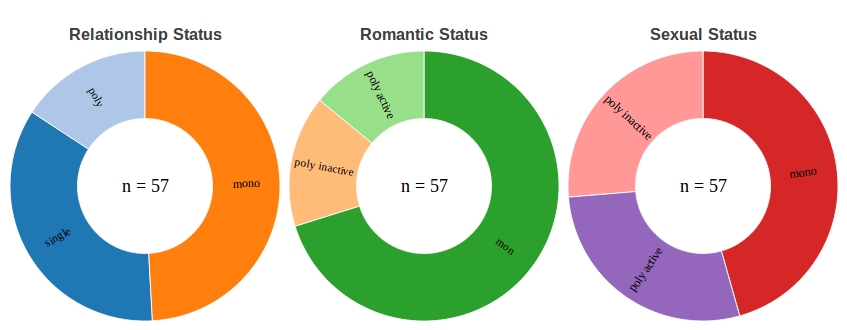
\includegraphics[width=\textwidth]{content/assets/polynormativity--results}
  \end{center}
  \caption{Monogamy/Polygamy survey results}
\end{figure}

Comparing these two gives us a few interesting points, in isolation:

\begin{itemize}
  \item Twice as many furries self-report as polysexual than as polyamorous.
  \item Three times as many furries report as polyamorous than in mainstream society.
  \item Twice as many furries self-report as polysexual than in mainstream society.
\end{itemize}

An interesting aside: before writing this article, I did an informal Twitter poll of ``do you identify as monoamorous or polyamorous, and why?'' The results, though I only got about two dozen responses, closely mirror the results of the [a][s] survey, which is great. The body of respondents very likely does too, in that, of n responses, n-1 of them were from furries. My follower ratio is slightly less furry-tilted than many that I know, at about 70/30 furry/non-furry, so we can informally posit that furries are also more likely to talk about these things, too.

To move on, I'd like to see what we can explore from the points we gleaned earlier.

\subsection*{Being a furry conditions us to think that polysexuality is more normal than the mean.}

Recently, I was at a friend's place for a weekly thing. The attendance list was ``eight furries'', as it usually is, plus or minus a few, but the point is, this is an event where furry social norms are in full force. Everyone greeted everyone else with a hug, there were 16 names for 8 people, all that jazz. At some point during the night, one of the attendants groped me. It wasn't incredibly invasive, as these things go: I told him to stop, people looked uncomfortable for three or four seconds, and that was that. He apologized, it didn't happen again, and all was good.

The interesting part of that event wasn't the event itself, but the discussions of the occurrence that happened after.

The host: ``This is why I wish that I had some more non-furry friends.''

This is a sentiment that I hear with alarming frequency, and could probably get its own entire [a][s] article. In general, it's assumed that furries are hypersexual, or at least more sexual than the average bear. This is also true of our assumptions of how the outside world sees us (ref), and statements like the one above do absolutely nothing to dispel that. ``Well, if it had been a group of you and seven other random non-furry people, they wouldn't have assumed that you were okay being touched.'' The idea being put forth here is that, as a group of furries, physical contact is expected, and therefore, we've normalized it to the point that a random grope is as mundane as a handshake is to someone outside fandom.

This is an unfortunate supposition. After all, a person who expects his personal bubble to be maintained would be offended regardless of whether or not the person doing the bubble-bursting happens to be a furry or not. Attempting to legitimize it as ``a furry thing'' does active harm to the outside perception of the fandom as oversexualized. It also does no real good for the furs inside who would prefer a more typical set of rules of engagement.

Submitted as Exhibit B: A friend who wasn't there said to me after the fact: ``Yeah, people do that to me all the time, because they assume that it's okay if I'm in a furry space.''

\subsection*{Being a non-furry operating in a mostly-furry space can skew one's perception of norms}

It's easy to see how this would be the case, but let's explore this a bit further. First, the social component: non-furries and furries alike accept the ``multiple name'' social construct to varying degrees. Personally, I attempt to find out a person's real name relatively early to avoid conversational awkwardness, as I would prefer to never have another conversation with my mother in which I have to explain why I don't know the name of the person who's crashed on our couch for three days. For a non-furry, this is even worse, as ``We spent the day with my boyfriend and his friend, uh\ldots Sheppenwolf\ldots '' is a risible statement in a great many contexts.

If we advance the clock a bit, it's easy enough to see how one can become immersed in this culture and normalize it. I, and by extension much of my social circle, have two friends that have legally changed their birth name to their furry name. Both have furry names that aren't readily identifiable as such, so it works, but in the event that they were named ``Tikkamasalacat'' or somesuch, a lot of people would shift readily. After all, we're used to using fan names as a primary mark. Mainstream society, not so much.

This translates very easily into the sexual side of the fandom, which I will discuss\ldots now.

\subsection*{Being a monogamous furry can lead to conflict with the fandom's polynormativity.}

This is something of a logical extension of the previous two, but it's worth touching on separately. At least one close friend of mine is strictly monogamous, and has expressed some discomfort at some of the standard furry social norms outlined above. This is a slightly extreme example, of course, but many people assume that it's okay to hug everyone they see at any sort of gathering, without actually asking. This probably shouldn't be the case, but many furries say that this is one of the things that they like about the fandom. Even so, one person's idea of openness is another person's idea of a popped personal bubble.

This bubble-maintenance can actually lead to some very interesting emotional backlash. Perhaps a monogamous furry feels as though he's cramping the style of the stereotypical furry by shying away from physical contact, or that maintaining monogamy is somehow counter to what the fandom wants or expects. I certainly went through a bit of this myself: early in my exploration of polyamory, I felt very weird for wanting to expand past my relationship, and that quickly evolved into ``but most of the people I know have multiple partners, so maybe I'm just doing this wrong.'' For what it's worth, while most of the people I know do in fact have multiple partners, or have at least experimented with such, this is just selection bias, even within the fandom.

There's an interesting thing to explore hiding in there, too: how 25\% became widely perceived to be a majority. Clearly, it isn't, but much like ``every man in the fandom is gay'', the assumption is often made that if you aren't naturally promiscuous, this fandom is not the place for you. There are a few possible explanations for this, at least some of which are erroneous assumptions in their own right: compare, for example, the perception that all of the art on FurAffinity is porn. It's actually somewhere around 23\% (ref), and that's ``mature'' and ``adult'' art \textit{combined}, but the fact that this is the art that gets the lion's share of the views and favorites means that the perception remains that furries are a lascivious bunch. Even if ``only'' 25\% of the furries are in open relationships, they're sometimes more vocal and certainly more visible, and that makes one more likely to think in terms of absolutes.

To conclude: the fandom's polynormative nature makes sense as an extension of its openness in other ways. We have a drastically higher percentage of people who see a hug, rather than a handshake, as the standard greeting. I would also argue that the significantly higher favorite count on adult art means that people are often not viewing it in shame. So it's pretty easy to extrapolate that to the conclusion that people who are open in general, as well as open about what they like, will be more likely to go seek that out.

The last thing to remember is that, while we are statistically more open than others, that doesn't mean that consent isn't still of paramount importance. Play safe, and communicate, just like you would expect to do within your relationship, and everyone can get along just fine.

  \articlehead{Why Zoophilia is a Furry Issue}{JM}{2013}

Zoophilia is fairly visible within furry.

Most obviously, so-called `feral' art is ubiquitous, and some animal characters -- the cast of The Lion King comes to mind -- seem to be minor sex symbols in some circles. More personally, furries sometimes actively denote themselves as zoophiles in social media, perhaps on their Fur Affinity page.

Klisoura's Furry Survey, which at its peak received over 9000 annual voluntary responses from furries worldwide, shows that 13-18\% of furries self-identify as zoophiles. This does not mean that all these furries have had sexual contact with a non-human animal; these furries are probably just reporting sexual attraction. However this is significantly higher than the general population.

Little research has been performed on zoophiles. Serious attempts to study the phenomenon are limited to the last ten years or so, at a level that academics compare to analyses of homosexuality in the 1960s (ref). All of these newer studies rely, in part, on Kinsey's landmark 1948 study, Sexual Behaviour in the Human Male (link) for data on the incidence of zoophilia.

Kinsey estimated that 6\% of American men have sexual contact with a non-human animal during early adolescence. The overwhelming majority of these cases were in rural areas. Such contact later in life quickly becomes vanishingly rare.

(There have been other studies, but none of any consequence. Notoriously, Alvarez \& Frienhar—ref—in 1991 reported rates of bestiality within the general population of 10\% to 15\% however this was based on a pitiful sample size of 20, all psychiatric staff.)

Kinsey attributes cases of sexual contact with non-human animals to young men lacking an available human partner. This is known as `situational sexual behaviour': sexual behaviour that takes place because of a dearth of otherwise preferred options. Such situational sexual behaviour is not limited to zoophilia. There are many other examples, gay sex in prison probably being the most obvious.

Like prison, situational homosexuality is common in gender-segregated communities. Gay sex is endemic in the armed forces of countries that have compulsory military service, Iran and Saudi Arabia in particular (ref). (The Singaporeans have a particularly unusual way of managing homosexuals in their National Service: openly gay men are given restricted duties that depend on whether they are `effeminate' or `non-effeminate'. Straight but effeminate men, or otherwise nonconforming men, are also given special duties. I like to imagine that there are whole platoons of drag queens in the Singaporean army, possibly defending Orchard Road from last season's shoe fashions.) Homosexual behaviour between young heterosexual men is also widespread in Muslim East African nations (notably Sudan) and single-sex boarding schools (notably England).

Situational homosexuality occurs inside the male-dominated furry community too. I've written a full article looking at the availability of men (and unavailability of women) within furry -- It's Raining Men -- detailing the plight of the heterosexual male furry. Suffice to say that their options are limited. Furry is an open environment that fosters intimate friendships (regardless of sexual preference), so it's not surprising that many heterosexual young furries will engage in mutually enjoyable sexual contact with male friends. The blunt categories of `gay' and `straight' are not strictly applied in the furry world (like they are in general society), so a heterosexual can engage in same-sex behaviour without risking the ire of his peers, or provoking an unresolvable identity crisis.

Situational bestiality also occurs within furry, partly due to furry zoophiles making their animals available for sexual contact. And, as Kinsey showed, it's common for young men with access to non-human animals to sexually experiment during adolescence. Further: frank depictions of zoophilic activity are easy to find in the furry community, as is frank discussion on the topic. Given this availability, it's inevitable that some young male furries will explore this side of their sexuality.

Kinsey's estimate of the numbers of adolescent men having sexual contact with non-human animals (6\%) was published in 1948. This was widely considered to be out of date by the mid-1970s (ref) and is even less relevant today. The reason for this is simple: we live in better connected and more sexually liberated society. The sexual revolution significantly improved the availability of women (and men) for young men; the proportion of people living in rural areas has declined; the spread of television provided a homogenizing influence on moral behaviour; the internet has significantly improved the connectedness of rural communities. The preferred mode of sexual contact is more available to more people, so situational zoophilia is much less common (ref).

Zoophiles today are different from Kinsey's farm boys. Those people engaging in sexual contact with non-human animals are much more likely to be pursuing it as a sexual preference. The number of zoophiles is small, and so congregation via the internet is common. The influence of the internet is the biggest difference between Kinsey's sample and today's zoophiles: the farm boys may have been influenced by a culture where sex with non-human animals was common, however this did not define the community (ref). Today's zoophiles congregate on the basis that their sexual orientation is an important part of their identity (ref).

And that's fair enough. Recent research strongly suggests that zoosexuality is a legitimate sexual orientation, a conclusion reached for homosexuality only in the late 20th century. I've written an article on this topic here on [adjective][species] -- Zoophilia in the Furry Community -- so I won't repeat myself. In short, studies over the last decade show that zoosexuals meet the requirements for a legitimate orientation in terms of sexual preference, fantasy behaviour, and love and affection (ref).

Zoophilia as a sexual preference will apply to some of the 15\% (or so) of furries that self-identify as zoophiles. As I mentioned earlier, this question was probably interpreted by most responders as relating to sexual attraction only. This isn't the common definition outside of furry: non-furry zoophiles tend to differentiate between `bestialists' -- those who engage with non-human animals for sexual gratification only -- and true zoophiles, who are concerned with welfare, perceived consent, and the sexual gratification of the animal (ref). However some of the furry 15\% will meet the definition of zoophilia as a sexual orientation, and this number will be significantly higher than the general population, optimistically estimated to be 1\% (ref).

Zoophilia is therefore a furry issue because zoophiles are a significant and visible part of our community. Like other unusually prevalent features of our community, as explored here in [adjective][species] -- homosexuality, Asperger's syndrome, fluidity of gender, online relationships -- the presence of zoophiles helps create and inform the wider furry culture.

Researchers into zoophilia have also made a connection: furry is included as a subset of zoophilia under a classification system proposed in 2011 (ref). Furries are specifically included as `Class I Zoosexuals', along with other people who engage in psuedo-zoophilic human-animal roleplay (e.g. pony play). Alarmingly, the author suggests that furries might be `treated' through behaviour modification therapy.

Fortunately, doctors and therapists are very accepting of unusual sexual behaviour. Even in the event that the classification of zoophilia formally includes `members of the furry fandom', it's highly unlikely that any form of treatment would be administered by a halfway-competent doctor or therapist. As things stand today, treatment is not generally recommended for any zoophiles (or other paraphiles). Any furry, or zoophile, seeing a therapist with a different opinion should strongly consider finding a new therapist.

\begin{quote}
  A final disclaimer: I am not a zoophile. I have never had any sexual contact with non-human animals and I've never had any desire to. This disclaimer serves two purposes: (1) I don't want to be subject to the abuse that zoophiles are often subject to; (2) I don't want this article to be seen as self-justifying. Thanks for reading. It's not an easy topic.
\end{quote}

  \articlehead{First Cons and Consequences}{Rabbit}{2013}

It's often said that the worst day fishing is better than the best day working. In my life, the same can generally be said of fur-cons. While I haven't kept actual count I've probably been to fifty or seventy of the things, and am fortunate enough to financially be in a position where, if I have a weekend off and there's one within driving range, I can usually go. I consider Mephit to be my ``home'' con, and that probably says a lot about my taste in conventions. I prefer them small, intimate and inexpensive. While I've been to and enjoyed Anthrocon several times and will probably eventually be back, well\ldots I don't know. Compared to the small cons the large ones feel impersonal. Commercialized. More about flash and gee whiz and Big Name Furs than ordinary people sitting around and making new friends.

Back when my columns were posted in other venues I sometimes wrote reviews of this and that con. Then I ceased doing so when I realized that these columns were garnering me a sort of ``VIP treatment'' that I didn't seek. (About the third time the chair of a con looked me up to ``make sure I was having a good time'' I sort of figured it out. And sure enough, when I quit writing these reviews the con-chair visits ceased.) All I want at a con are reasonable prices, ideally between twenty and three hundred furs to interact with (preferably a few of which I already know), a couple-three fursuiters running around from time to time, and some good (preferably writing-related!) panels to go to. The rest sort of takes care of itself, and most cons are well advised not to mess too much with this winning formula.

I've always been especially interested in attending ``first-time'' cons. There's an extra-special sort of magic at these, as a rule -- even the things that go wrong usually just add more ``flavor''. I suspect this is because first-time cons have first-time con staffs, for the most part, who are fresh and unjaded and eager to make ``their'' convention work well. (I was at the first Rain Furrest, the first Furry Fiesta and I think the first MFF, among several others.) Everything is new and exciting to everyone, including many of the attendees, and a sort of magic fills the air.

Usually.

I have seen first-time cons crash and burn, however. It takes work, but I've seen it managed. So I'll complete this column by telling a few woeful tales and offering advice.

\subsection*{1) Registration}

The very first thing congoers experience of a con is Registration. Organizing all those badge sales is difficult, low-profile work performed by people who are in most cases going to miss large slices of the con as a result. (I try to make it a point to recognize whoever registers me for the thankless role they've volunteered to accept.) Sometimes poor Registration experiences are inevitable -- computers crash, printers fail, etc. But, what's not inevitable are gross social and customer-service errors. I recently had the worst Registration experience of my life, when I was left standing at the desk for at least three and perhaps as long as five minutes while the Registration staff totally and completely ignored me even though I was the only one there. The staff spent the time chatting and working on some sort of craft-type project even though I was standing less than two feet away looking at them. Finally, at long last, the person sitting opposite me asked what I wanted. ``To buy a registration,'' I responded.

Their eyes went wide. ``Oh!'' they said. ``I thought you were with the (tool-related) convention! You're wearing a work shirt!'' Then they proceeded to ignore me again for at least two more minutes.

And so, because I was wearing a work shirt (and probably because I'm a good bit older than most con-goers) I started this con off on a totally bad foot. So bad, in fact, that for the first time ever I resolved to inform the con chair about how badly things were being run in Registration.

Then, a little later, I learned that the con chair was the person who'd ignored me.

Which leads well into Point Two\ldots

\subsection*{2) The con is about the attendees, it's not about the staff or the Guests of Honor}

I attended both opening and closing ceremonies at this same con. I usually attend neither, as I generally find them boring. But this time I attended Opening Ceremonies in order to learn what the Con Chair looked like, and then Closing for the same reason that one gawks at a car wreck. At both events the speakers attempted to improvise instead of working from set notes, and the resulting chaos was all too predictable. In the end little to no useful information was transmitted. The staff spent most of the time referring to and congratulating each other instead of interacting with the attendees. They spend some time tossing candy/whatever into the crowd, but the products were thrown hard enough (and some were heavy and sharp-edged enough) to cause potential injury. Several of us attendees -- total strangers -- met each other's eyes and shook our heads at each other; it wasn't just me who disapproved. Apparently, pretty much everyone understands that blinding your guests is a poor way to begin a con.

Another thing I've sometime seen at cons, though not this specific one I've been citing, is a GOH who does their best to sabotage the proceedings. I've seen GOH's do truly awful things, like get so drunk that I've personally had to give multiple panels for them. But worst of all is when a GOH gets the idea in his or her head that the attendees are there for them instead of the other way around. A GOH, in my opinion, owes an even greater debt to the con and its attendees than any staff member save perhaps the Chair him or herself. They're being honored in a unique and what should be humbling way. GOH's shouldn't just be willing to provide art/stories/whatever. They should actively make an effort to circulate, shake hands, and for heaven's sake show the unwashed masses that they're pleased to be honored! Good GOH's can make even a mediocre con memorable. Poor ones can make a wonderful con disgusting. Therefore, it's essential they be selected carefully and have a clear understanding of their vital role.

\subsection*{3) The Hotel Employees}

It's natural that the hotel employees, especially for a Year One con, should stand with wide eyes and be amazed at the wonderful weirdness of it all. They're part of the con too, so why should they not enjoy a little of it? Indeed, I try to take the time to speak with them in a friendly way and explain what I can, when I can. Con Staff should absolutely do the same at every opportunity. Perhaps it's because I'm blue-collar myself and therefore I'm extra-sensitive to such things, but I don't often see Staffers interacting with the hotel workers in a fraternal way. People may not be aware of this, but when they give snippy, hurried instructions to someone they assume ipso facto must be stupid or they wouldn't work at a hotel, well\ldots It's insulting as hell. This doesn't so much cause problems for a Year One con as it does down the road after repeated exposure, but I mention it here anyway because it needs to be dealt from the very beginning.

Hotel workers may be low-paid, but they're intelligent, sensitive fellow human beings asked to keep a straight face at some pretty outlandish stuff. They've got full, rich lives and interests of their own. At one con, for example, I met a waiter originally from New Orleans who had personally met most of the biggest names in Jazz, was probably a bonafide expert on the subject (I'm not qualified to say) and kept a huge private music library. Such individuals deserve as much respect as any congoer. Again, as a blue-collar guy myself I'm uniquely positioned to note that it doesn't help in the least when the person being snippy is half their age. And I'm also uniquely positioned to inform you that payback can be hell.

Trust me. You'll never regret making friends in low places. Especially at con hotels.

\subsection*{4) Programming}

It's incredibly tough to set up programming at a first-year con. Usually there are few rooms available, and often even fewer credible Subject Matter Experts. I always prefer more panels at a con rather than less, on the grounds that then I always have something interesting to do. Therefore that's what I suggest to the first-year programmer. A poor panelist, so long as they're polite and civil and smile a lot, is generally better than no panelist.

On the same note\ldots don't ever ask a panelist to share a room with another panel, or give a panel in a place like the Hospitality Suite. You're asking the impossible in such a chaotic environment.

\subsection*{5) Atmosphere}
This one's tough, but I'll give it a shot anyway. I don't know about others, but I can walk into a room full of people and in a matter of seconds know if they're bored, happy, hostile or whatever. If you think about it, a very large part of the con experience takes place in the meeting rooms and other public gathering places. It doesn't take a con staffer, especially the chair, two minutes to physically go to these places, ``sniff the air'', and then if necessary do something to improve the situation. He might ask a GOH fursuiter, for example, to swing by the gaming room if it's ``dead''. Or, if the ``social'' area looks slow, he might sit down and chat with a few individuals, smiling frequently. Atmosphere is an elusive thing, yes. But you don't have to be passive and accept whatever comes. Go out there and do something about it!

And that's pretty much it, I suppose -- Phil's take on How Not to Totally Screw up a First Con. I hope someone, somewhere has a better time for it having been written.

  \articlehead{The Science of Zoophilia}{JM}{2013}

Scientific research on human sexuality is a relatively new field. The Kinsey Reports, published in 1948 (men) and 1953 (women) (link), were the first attempt to gather data on human sexual behaviour. These were informally updated by Playboy in the 1970s (link), back when it retained some literary relevance, in an attempt to understand the changes brought about by the sexual revolution, and -- of course -- to provide some salacious reading material.

It took until the early 1980s for researchers to confirm that homosexuality is largely set at birth (ref). This work, controversial at the time, contradicted the prevailing wisdom that male homosexuality came about due to feminization of a male child, caused by an overbearing mother and distant father (the reverse supposedly applied for lesbians). This conclusion was simple enough to make: researchers interviewed a large number of people, asking about their childhood and sexual preference, then looked for correlations. (They found none.) And yet such simple data gathering took more than 30 years after Kinsey to be published.

The science of zoophilia is much less mature. Kinsey asked questions and gathered data (as did Playboy) however the first serious attempt to understand zoophilia was published more than 50 years later, by Dr Hani Milestki in 1999. Miletski's book suggested that zoophilia may be a legitimate sexual preference: one defined by love, not sex.

Miletski's book was followed by research from two long-time specialists in the field—Drs Williams (wikipedia profile) \& Weinberg (wikipedia profile), who started their careers studying homosexuality in the 1960s. (Weinberg, literally, wrote the book—in 1981—that showed that homosexuality was set at birth.) The two are highly respected in their field, and their results agreed with Miletski when they published in 2003. Research into zoophilia has increased since then.

(The works of Miletski -- \textit{Understanding Bestiality and Zoophilia} -- and Williams \& Weinberg -- \textit{Zoophilia in Men} -- are \sout{available in full for free, and are} barnstorming reads. They are both recommended, Miletski in particular, although you'll want to gird your loins for some vivid language.)

The two works are notable for going beyond analysis and discussion of statistics: the authors clearly became sympathetic towards the zoophiles during the course of their research. This sympathy isn't evident in the results, but it is evident in their discussion of the zoophile lifestyle. They note that the zoophiles face unusual personal and ethical challenges as a result of their taboo sexuality. Williams \& Weinberg make a direct comparison with the subjects of their early work, homosexual groups in a less tolerant era:

\begin{quote}
  They reminded us of some of the early gay groups we studied in the 1960s and 1970s, especially when they engaged in banter about sex (in this case, it was not just sex with men).
\end{quote}

Homosexuals in that era were seen as dangerous sexual deviants, similar to the way that zoophiles are seen today. However it is very clear from the results presented in Miletski and Williams \& Weinberg that the relationship between a zoophile and his/her animal partner is based on love, where sex is an expression of that love.

This brings about a special problem faced by zoophiles: if you are in love with a non-human animal, where do you find human contact?

This is clearly a significant personal challenge for the zoophiles, especially given that they must hide their taboo sexuality from most people. Many zoophiles displayed a tendency to anthropomorphize their animals (ref Williams \& Weinberg):

\begin{quote}
  When asked “Is being in love with an animal different than with a human?” approximately three quarters answered positively. The features the men mentioned were anthropomorphic in that they described ideal human love relationships. Ironically, humans were often seen as less able than animals to provide those ideal human characteristics.
\end{quote}

This is a special kind of misanthopy, one where human emotions are projected upon an animal to create an ideal that cannot be met by a real human. This false creation of a perfect, or near-perfect, oxymoronical hyper-human non-human is only going make it more difficult for a zoophile to find real human contact.

Humans are social beings. We have evolved to need one another's company, and we communicate in subtle ways that meet our social needs. A relationship between a human and a non-human will always be one-sided, regardless of the perception of mutual love.

The zoophiles can end up with an unhealthy misanthropic perspective, a perspective I would compare with that felt by depressed people:

\begin{quotation}
  I find the company of animals more pleasing than that of humans – there's less stress, fighting… Love with an animal is how love should be – a lot less complicated with no strings attached. (Williams \& Weinberg)

  I can identify with dogs a lot more than I can identify with humans. I am thinking a lot like dogs, and therefore I can understand dogs better than humans. (Miletski)

  I felt I could only trust animals. They didn't gossip, they didn't laugh at me, they were available most any time. (Miletski)
\end{quotation}

In these comments you can hear the reflected neuroses of the zoophiles. They feel that humans cannot possibly live up to their expectations, or that they themselves will fail to `fit in' with society, so they regress and find reasons to avoid people altogether.

Marcel Proust, as ever, intuited this, framing depressive misanthropy as a reaction to a need to be part of (an untrusted) society. The following quote is from the second volume of \textit{In Search Of Lost Time}:

\begin{quote}
  In a recluse, the most irrevocable, lifelong rejection of the world often has as its basis an uncontrolled passion for the crowd, of such force that, finding when he does go out that he cannot win the admiration of a concierge, passers-by or even the coachman halted at the corner, he prefers to spend his life out of their sight, and gives up all activities which would make it necessary to leave the house.
\end{quote}

The sad irony is that those who have the least social contact are the ones most in need of social contact.

The other issue is, of course, the ethics of sexual contact with a non-human animal. Animal sexual abuse can sometimes be a problem (ref), and such behaviour is commonly assumed to be the act of a zoophile.

According to the researchers, making a connection between zoophilia and animal abuse is wrong. The zoophiles were defined by their love for the animals. Miletski states:

\begin{quote}
  The majority of my subjects love their animal-partner. Some see them as a spouse and will do anything for them. Sexual relations with the animal is an expression of love for them, and if the animal tells them, with its body language, that it is not in the mood for love-making, the majority of my subjects will leave the animal alone. In fact, many of them are members of the Humane Society and other organizations that are taking care of animals.
\end{quote}

The ethical issues associated with zoophilia are important however I don't intend to explore them in detail here. This is difficult ground because of the strong moral reaction people often have to zoophilic acts (very comparable to the strong moral reaction some people have to homosexual acts). In general, researchers and ethicists on the topic (notably Peter Singer, author of \textit{Animal Liberation}, ref) agree that the issue is whether the animal is harmed, and that the sexual aspects are irrelevant. This may be the subject of a future article (although, given my recent article on Why Zoophilia is a Furry Issue I'm a bit concerned about turning [a][s] into \textit{Zoophilia Weekly}).

There is a small zoophile subculture growing on the internet. Zoophiles are expected to continue to congregate online, due to their small numbers and the benefits of anonymity. Many of them, including some who participated in Miletski's study, have engaged with the furry community. This makes sense: furry provides what is important to zoophiles, namely a largely online-based culture with strong social connections, an emphasis on intimate friendships, and a safe environment for people of unusual sexual or gender orientations.

It's no accident that the researchers compare zoophiles today with the GLBT community of 50 years ago. Gay relationships were seen as an exercise in immoral sexual behaviour, however this has changed as homosexual relationships are now largely perceived to be about love. The zoophiles have not reached this stage, but they may find that the furry community provides a social environment where their love is tolerated as unusual but acceptable. If zoophiles can be open within furry, they can provide good role models for the `zoo-curious', helping young people manage and accept an otherwise complex and difficult sexual orientation.

I expect the level of conversation within the furry community to improve over time as the number (although perhaps not the proportion) of zoophiles increases. We will see more intelligent, respected, well-adjusted zoophiles be open about their orientation within furry. Dismissive and offensive language will become marginalized, just like homophobic language has declined in general society in recent years. And conversation topics, online and offline, will move away from the presumption of abuse, and towards the real ethical and emotional challenges of being a zoophile.

  \articlehead{Furries and Music}{Makyo}{2013}

Furries and music definitely have a thing going on. I've wanted to write about it for quite a while now, but I've never quite found the right entry point, the right way to piece together a story about how the two might connect. I actually started thinking about the current topic when Klisoura of Furry Survey lore was in town over the week between Christmas and New Years, and the topic came up of how furries have a tendency to consider themselves ``ahead of the curve'' when it comes to music, television, and video games, or even trying new things, yet do not necessarily consider themselves to be hip or paragons of pop culture (ref). While I'm really as much of a fan of new music as anybody out there in this subculture, I wasn't quite sure how well this held up. What the data seem to be saying is that furries showed a tendency to eschew popular culture in favor of the type of things that would become popular culture. While some of our number may fit within that category, it's oddly specific for a subculture that doesn't, at its roots, have as necessary an intersection with popular culture as might, say, the fans of an actual genre of music, television series, or video game.

A survey is a survey, though, and can only really tell so much about those who really should be telling the story. I turned, instead, to Twitter, and invited an email barrage on myself to see what those who had the stories to tell had to say about the matter, asking ``Do you think furries are more or less musical than non-furs?'' and ``Do you think furries are ahead of the curve in terms of music?''.

Let me take a step back and say that I've always been kind of fascinated with the relationship that furries have with music. I spent the time and money (lots of the latter) needed to get a bachelor's degree in music composition, so I've always been, as I glibly put it on Twitter, super into music, and so I'd always wondered if maybe it was the crowd that I hung out with that was influencing my perceptions of furries as rather musically oriented folks, or if maybe it was just everyone. Another thing that piqued my interest, however, was the visible importance of music at conventions and in every-day chatter. The latter could be explained away by the fact that a lot of folks within furry aren't going to spend every second role-playing, of course, they're going to have conversations about the things that interest them, and music is a natural topic even outside the fandom. The former, however, intrigued me, even after I started regularly attending conventions. There were dances every night. There were dance competitions, dance competition try-outs, dance competition out-takes, dancing in the fursuit parade, dancing for no reason. Music seemed to be everywhere, from panels to the dealer's den, and it all made me pretty happy, if curious.

Furries, like everyone can be broken down into two, very rough, categories when it comes to things like music: creators and consumers. The act of creation plays a big role within the fandom, of course. Given that we are, as was famously put, ``fans of each other'', we rely primarily on our own membership to create the art and stories appreciated within our subculture. Within music, however, things are a little more gray. The question of whether or not there is such a thing as furry music and what might define it is one for someone else to answer, but needless to say, there are still plenty of furry musicians. There are several out there that create music within the context of furry, post their music to FA, or perform at conventions (such as the jazz combo SuperPack at FC a week and change ago). ``[T]he environment seems more conducive to the sharing of content in general, music included. Furry musicians have a built-in audience they can reach that many other aspiring artists might not.'' Vincent writes, and I think this is an apt description of at least part of the reason there is a music scene within our fandom, or indeed within many subcultures.

There's one more smaller subset we should probably take into account given the popularity of dances and the like at cons, not to mention the relative popularity of electronic music within the fandom, and that's the wide variety of furry DJs out there. The reasons for the popularity of this pursuit are varied, and hinted at by several of those who wrote back. Technological aptitude, diversity, a focus on sharing, and interest in EDM (electronic dance music) as trends within our subculture may help guide many toward DJing as a mode of expression, and notably as a way of sharing things important to themselves.

Beyond simply creating or creatively mixing music, though, we are avid consumers of music, at least commensurate with our strongest demographics. Soto writes, ``From a consumption standpoint, I haven't found furries to deviate much from their non-furry counterpoints in the same demographics. For example, age group. Furries as a whole may be more passionate about music and stay more current with trends, but furries as a whole have that lovely age-skew toward the late teens and twenties, and that age group is generally pretty up on their music as it stands.'' That is to say, we're helped along by some of the categories that many of our members belong to in listening to and exploring music with the sort of enthusiasm that goes along with connoisseurship.

So, what about my two questions? As hinted about in the previous quote, opinions are mixed on the question of whether or not furries are more musical than their non-furry counterparts. In fact, after reading many of the responses, I don't think the question should be whether or not furries are more musical than their counterparts, but whether or not they have the conception that they are. Zenuel offers, on the positive side, ``I like to think that the fandom simply offers more open and honest states of being[\ldots ]; a furry posts to a more receptive community like FurAffinity they generally receive more encouraging feedback, as well as having the backing of freedom that the fandom presents to the artist in question.'' Vincent acknowledges this, but warns, ``This is a pro and a con, I've always seen furry as something of a `hugbox' where criticism isn't forbidden, but it certainly isn't forthcoming. I've found that (at least in the realm of DJing) it's very, very hard to get good technical feedback on how to improve, and in many instances subpar mixing is lauded as exceptional.''

One advantage that we do have that we gain from being a decently coherent subculture is the fact that we are rather diverse in ways unrelated to some of our stronger demographics. That is, age and gender aside, our diversity in terms of backgrounds, social status, education, and so on does help us with the ways in which we deal with music. As Wolfdawn put it, ``just being part of a diverse and unusual subculture would have to be a big [plus], since that alone makes people more likely to have been exposed to wider range of musical interests as they're shared among friends.'' I noticed a similar effect outside of furry when I moved away from my rather homogeneous upbringing and high school to college, where much more diversity was to be found. College was where I expanded beyond my own choral background into genres, classical and not, far beyond what I was used to. Furry was much the same, and in fact, much of this article was written listening to a playlist composed almost entirely of music suggested to me by cats, dogs, and all sorts of fuzzy creatures. In other words, are we more musical than the non-furries that surround us? Probably not. However, do we consider ourselves more musical than those around us at least in part because of furry? Often times, I think so, and a lot of these responses echo that sentiment.

As to the second question, you'll note that I put ``ahead of the curve'' above in quotes. These weren't meant to be scare-quotes, necessarily, but I would like to highlight something before I get too far. It's always very important to pay attention to the ways in which language is used. I know, I write about words a lot (using, of course, as many words as I can), but when I responded to the onslaught of emails with the two questions, I tried to do so using language that would invite people to provide longer, rather than shorter answers, because I think that the thoughts of those being asked are much more interesting than simple yes-or-no answers on the subject. It's the way that people interpret the questions they're asked, sometimes, that provides a lot of the answer. I understand that ``ahead of the curve'' can be a little misleading in terms of being able to provide a concise answer, and I'm sure I could've worded it better besides, but the answers I received in reply more than made up for it in their thoughtful and well-put responses.

Are we ahead of the curve? A lot of folks who replied indicated that no, we're not really all that ahead of the curve, at least not moreso than we might necessarily be given some of our demographic skews. There are a couple of reasons behind this, and one of the big ones is that the Internet and mass media in general hasn't benefited only furries. ``The increased visibility of various scenes took away the relative advantage having a community that encourages sharing,'' writes Vincent, and this is echoed by a lot of my own perceptions: my composition professor went on a `where is the drop?' joke spree with almost all of his students once dubstep became a more visible part of the music scene around us (the idea of being separate, here, due mostly to the fact that we were being classically trained in composition). That aside, however, Branwyn suggests that many ``are in the same arena as non-furs -- they consume music in the same way, influenced by the same sources, regardless of quality.'' That is, being furry does not necessarily influence the ways in which we appreciate music, so much as some of the content that we listen to. We listen to the things our circle of friends listen to, in all probabilities, and I believe that much the same happens when it comes to visual art, for that matter; we don't enjoy visual art that much differently (though we do sometimes place quite a bit of importance on a visual representation of a character -- ref), so much as enjoy the things that our chosen family and circle of friends also enjoy.

A possible explanation for all of this is offered by Forneus: ``Furries are, I would argue, more musical than the mean, but not moreso than other geek subcultures.'' We are, of course, not the only subculture based almost solely around a shared, intense interest. The My Little Pony fandom has created a wealth of their own music, not to mention filking, which as a long and well-established tradition. Several of those who responded to the questions touched on the points of geekdom and technology, along with their ties to the fandom. One respondent talked at length about the fact that there are readily available tools on the market now, and, despite the fact that many, given such tools, will create music that might not be the best in terms of musicality and technical ability, they are still creating quite a bit (my own experiences with Reason are a testament to this, of course). ``I think that if you put the tools in front of furries, they are more willing to try creating music than regular people,'' echoes Nathaniel Hahn; this does well at pointing out the fact that, rather than being more innately musical or musically hip, we may simply be focused on putting something out there given the tools we have for our subculture to enjoy.

Satori sums it up well, ``We have geeks of all kinds, and some geek on their music. Others are too into geeking on other things that they don't make the time for it much.'' We're just us, in the end. We're a good mix of musical and non-musical fuzzies, no more or less of a mix than the world at large. We have things working to our advantage, such as our broad social circles, diversity, geekdom, the Internet, and so on, but no matter how large a part music plays within the fandom, we're still just us, and some of us will create, and others will consume. We're no less interesting for being a good mix, of course, and music does still appear to be quite important to us, but in the end, we're plenty good at focusing on being and appreciating animal folk.


  \chapter{February}

  \chapter{March}

  \chapter{April}

  \chapter{May}

  \chapter{June}

  \chapter{July}

  \chapter{August}

  \chapter{September}

  \chapter{October}

  \part{About the Authors}
  \section*{[adjective][species] Staff}

\begin{description}
  \item[Makyo] \textit{hosting; programming; writing; editor-in-chief} -- Makyo's been in furry under various names since sometime around 2000, running projects such as [adjective][species], The Furry Survey, and Characters @ Openfurry.  She is usually to be found pretending to be an arctic fox and working in the software industry despite her degree in music composition.
  \item[JM] \textit{horse} -- JM is a horse-of-all-trades who was introduced to furry in his native Australia by the excellent group known collectively as the Perthfurs. JM now helps run [adjective][species] from London, where he is most commonly spotted holding a pint and talking nonsense.
  \item[Klisoura] \textit{survey magic; sounding board; moral support} -- Klisoura helps run the Furry Survey, and provides insight on the results for [adjective][species]. His page contains more of his musings, and is hosted on the Soviet Union's TLD, how awesome is that?
  \item[Zik] \textit{fish procurement strategies} -- Zik is an otter who's been dabbling around the furry fandom for nearly a decade. When he isn't doing schoolwork, he spends time raging at videogames as well as hunting down music, art\ldots and fish.
  \item[Rabbit] \textit{derived from a failed design for a folding bicycle} Rabbit is the author of over twenty published furry novels and novellas as well as numerous columns and articles in other furry venues. He’s a Tennessee auto worker.
  \item[Kyell] \textit{writer fox extraordinaire} Kyell is a fox, a writer, and a California resident. He likes to write stories of varying lengths, often (but not always) dealing with gay relationships and foxes. You can find information about his stories on his website, and read his blog for thoughts on furry fandom, writing, gay rights, and eagles, and for information on his upcoming books.
  \item[Lunostophiles] \textit{Cheshire cat} Lu has been in the fandom since he was 14, though Cheshire cat only came about seven years in. He is a creator, both of writing and of fibre arts, and sometimes pretends he’s a musician. When he grows up, Lu wants to be a Time Lord, but until then, he’s masquerading as an advice columnist and pop culture polyglot.
  \item[Shining River] \textit{greymuzzle} Shining River lives in the high lands of Utah and began participating in the furry community in 1998. Besides furry art and literature, he is interested in Scottish and Irish culture and Western American folk culture and history. You may see him in public performing with one or two of our local Scottish bagpipe bands.
\end{description}

\section*{Guest Contributors}

\begin{description}
  \item[\ldots] \ldots
\end{description}


  \newpage
  \secdiv
\end{document}
